\chapter{Theory and Motivations}
\label{chap:theory}


%\chapterquote{I may not be there yet, but I am closer than I was yesterday}
%{Unknown}

%% Note that the citations in this chapter use the journal and 
%% arXiv keys: I used the SLAC-SPIRES online BibTeX retriever 
%% to build my bibliography. There are also quite a few non-standard
%% macros, which come from my personal collection. You can have them
%% if you want, or I might get round to properly releasing them at 
%% some point myself.

\chapterquote{Absence of evidence is not evidence of absence.}
{Carl Sagan, 1934 -- 1996}%


This chapter introduces the \ac{SM} as a gauge invariant \ac{QFT}, and gives a description of the fundamental particles and their interactions.
The shortcomings of the \ac{SM}, outlined in Section~\ref{th:BSM}, imply however that it must be an incomplete description of nature. 
A Supersymmetric extension of the SM can address many of these limitations and is described in Section~\ref{th:SUSY}. 
Particular emphasis is placed on the arguments for \ac{SUSY} with compressed mass spectra in Section~\ref{th:CMPsusy}, as this is the subject of this thesis.
% The convention $c=\bar{h}=1$ is used throughout. 
% The four vector indices are labelled $\mu$ and $\nu$.
% The $SU(2)$ generators are labelled $i$, $j$, and $k$, while the $SU(3)$ generators are labelled $a$, $b$, and $c$.
%Gravity, of order $10^{33}$ times weaker than the forces discussed in this chapter, is neglected.
%The lack of any explanation of gravity within the \ac{SM} suggests its incompleteness as a total description of nature.

\section{The Standard Model of Particle Physics \label{th:sm}}

The \ac{SM} of particle physics provides a fantastically accurate description of the fundamental particles of nature and their interactions via the strong, electromagnetic, and weak forces at the electroweak energy scale.
It has proved itself incredibly robust during the first years of \ac{LHC} running. 
Many high precision measurements of production cross sections (which can be understood as the number of events produced) are consistent with their loop level \ac{SM} predictions, see Figure~\ref{fig:stairwayToHeaven}, 
which shows many different experimental measurements and theory expectations agree over 6 orders of magnitude.
Even very rare processes have been measured to agree with their \ac{SM} predictions: the decay $B_{S}\rightarrow \mu\mu$, very sensitive to new physics processes, has been observed at the level of three in every billion decays of the $B_{S}$ meson~\cite{BSmumuCombo}.
Such tests of the \ac{SM} cement its place as one of the major successes of 20$^{\rm th}$ century physics.


\begin{figure}[htbp]
  \begin{center}
  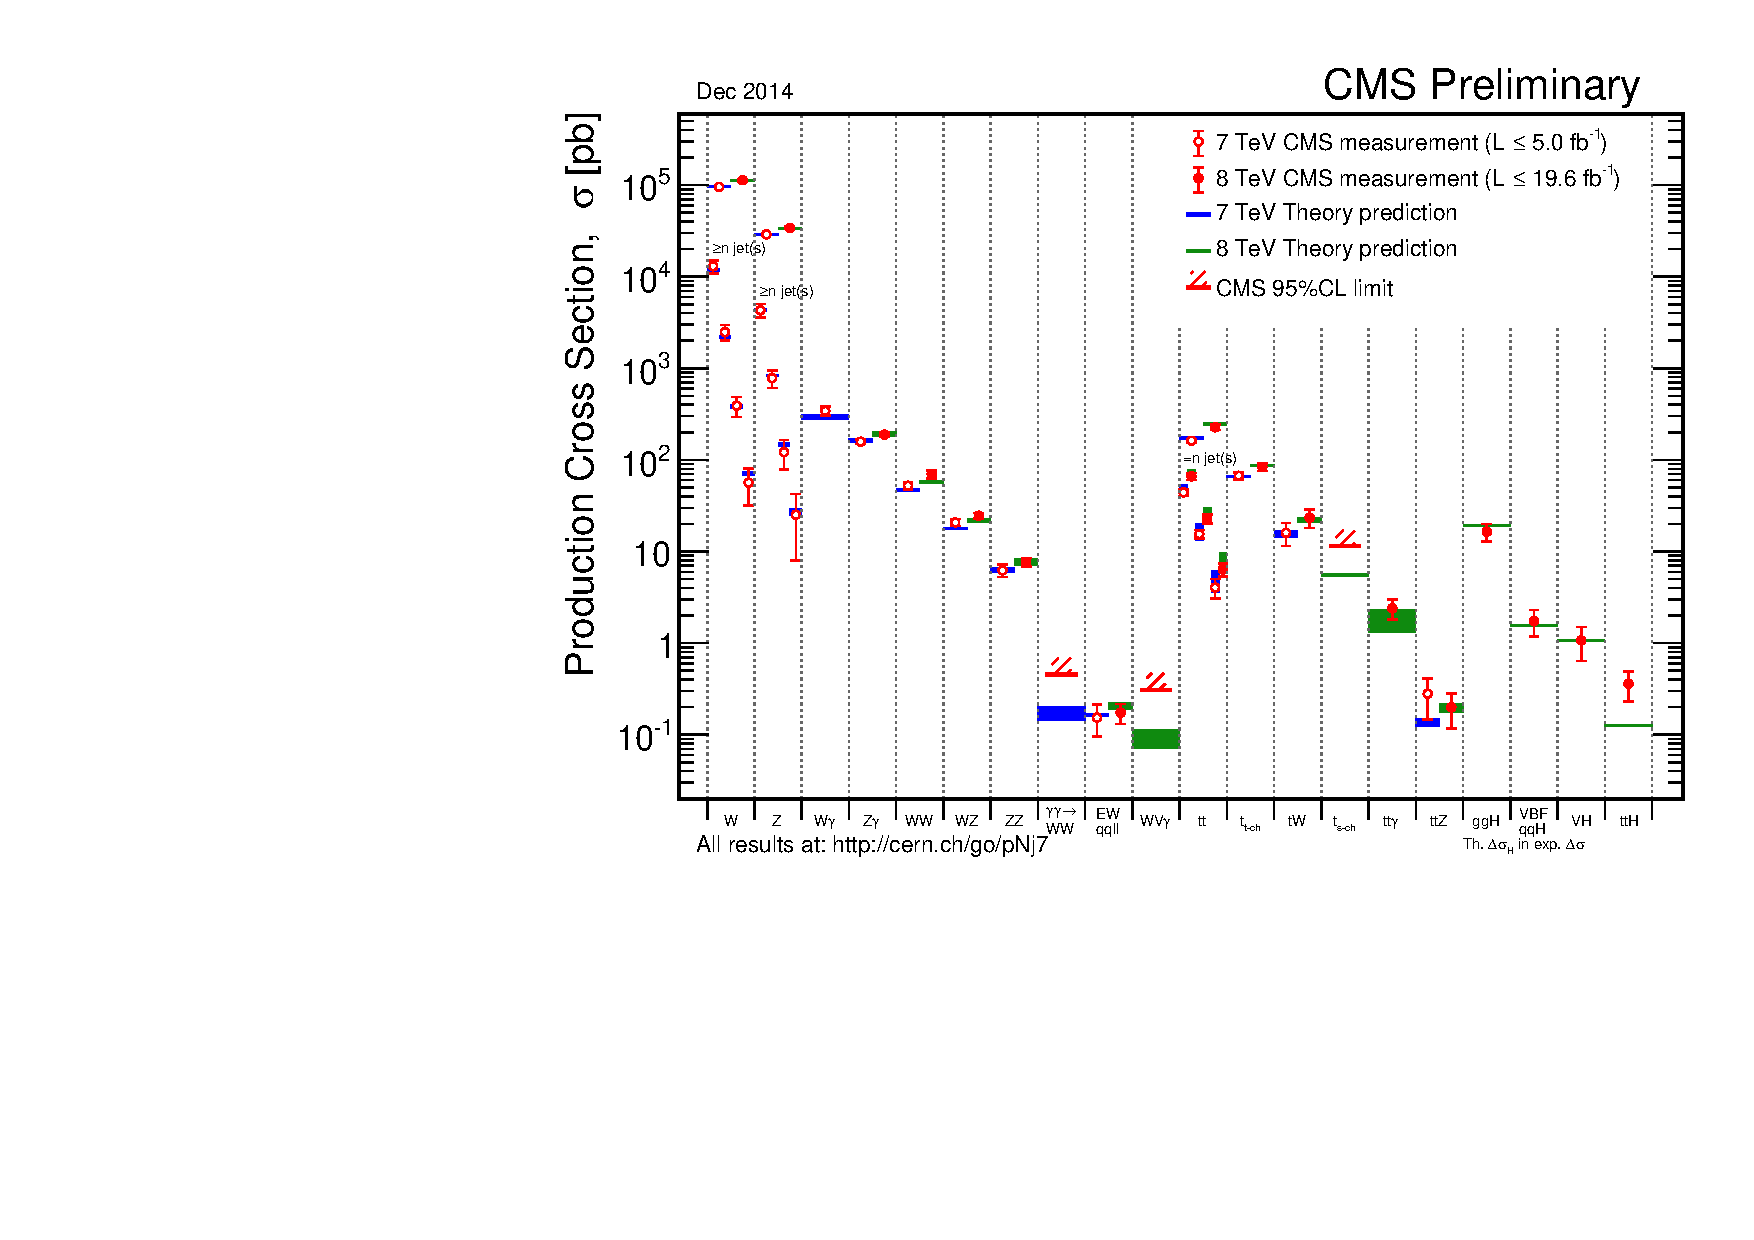
\includegraphics[width=0.8\textwidth]{Figures/theory/SigmaNew_v0}
  \caption{Combined results from \ac{CMS} of many \ac{SM} measurements made at \ac{LHC} centre-of-mass energies of 7 and 8~\TeV, taken from~\cite{CMSpublictwiki}. Theory and experiment agree over a vast range of production cross section values, for many different \ac{SM} processes.
}
  \label{fig:stairwayToHeaven}
  \end{center}
\end{figure}

Developed in the 1960's and 1970's~\cite{PhysRevLett.19.1264,Glashow:1961tr,Salam:1968rm,Hooft1971167}, the \ac{SM} is a relativistic \ac{QFT} in which particles are excitations of fields. 
It is gauge invariant, guaranteeing its renormalizability, and contains three symmetries:
$SU(3)_{C} \otimes SU(2)_{L} \otimes U(1)_{Y}$.
$SU(3)$ describes the strong force, felt by coloured particles, 
and $SU(2) \otimes U(1)$ describes the unified Electromagnetic and Weak forces, felt by particles with weak isospin and weak hypercharge. 
The Higgs mechanism~\cite{PhysRevLett.13.508} describes the spontaneous symmetry breaking of the $SU(2) \times U(1)$ gauge symmetry which allows for massive gauge bosons in a gauge invariant way.
The discovery of the Higgs boson~\cite{Aad:2012tfa,Chatrchyan:2012ufa} in July 2012, the mediator of the Higgs field, provided the last piece of the \ac{SM}. 
% Here, the subscript $C$ is for colour charge,
% $L$ is to signify only left handed fermions belong to the group, and $Y$ is for the Yukawa couplings which affect all matter.


\subsection{Fundamental particles and forces}
All known matter in the universe can be described by the fundamental matter particles, which can be separated into quarks -- those that feel the strong force, and leptons -- those that do not.
Matter particles are all spin-$\frac{1}{2}$ fermions that conform to Fermi statistics and obey the Dirac equation~\footnote{The convention $c=\bar{h}=1$ is used throughout and the four vector indices are labelled $\mu$ and $\nu$.}.
%
\begin{eqnarray}
\label{eqn:Dirac}
(i \gamma ^{\mu} \partial_{\mu} - m) \psi =0,
\end{eqnarray}
%
where $\gamma^{\mu}$ are the Dirac matrices, which are defined by their anti-commutation relation 
$\left\{ \gamma^{\mu}, \gamma^{\nu} \right\} = \gamma^{\mu} \gamma^{\nu} + \gamma^{\nu} \gamma^{\mu} = 2 \eta^{\mu\nu}I_{4}$,
where
$ \eta^{\mu\nu} $ is the Minkowski metric $(+, -, -, -)$, and $I_{4}$ is the four-dimensional identity matrix;
$\delta_{\mu}$ is the covariant derivative; and $m$ is the mass of the particle.
Repeated indices are summed over~\cite{HalzenMartin}.

A summary of the matter particles of the \ac{SM} can be found in Table~\ref{tab:SMfermions}. 
A similar table exists for the antiparticles of the leptons and quarks, a consequence of Equation~\ref{eqn:Dirac}, which has both positive and negative energy solutions. 
Rather than particles travelling backwards through time, as the negative energy solutions suggest, anti-particles are interpreted to have all of the same properties as their partner particles but with opposite charge.

\begin{table}
%\footnotesize
\begin{center}
%\begin{tabular*}{0.75\textwidth}{@{\extracolsep{\fill}}c|ccc|ccc}
\begin{tabular}[ht!]{c|ccc|ccc}
\hline
\multicolumn{7}{c}{Matter fermions: spin-$\frac{1}{2}$} \\ \hline
 & \multicolumn{3}{c|}{Leptons} &\multicolumn{3}{c}{Quarks} \\ 
Generation & Particle & Mass (MeV) & Charge & Particle & Mass (MeV) & Charge \\ \hline
\multirow{2}{*}{1} & $\nu_{e}$    & $\sim0$    & 0  & d & 2.3  &$-\frac{1}{3}$\\
 				   & $e$          & 0.511& -1 & u & 4.8  &$+\frac{2}{3}$\\
\multirow{2}{*}{2} & $\nu_{\mu}$  & $\sim0$    & 0  & s & 95   &$-\frac{1}{3}$\\
 				   & $\mu$        & 106  & -1 & c & 1270 &$+\frac{2}{3}$\\
\multirow{2}{*}{3} & $\nu_{\tau}$ & $\sim0$    & 0  & b & 4180 &$-\frac{1}{3}$\\
				   & $\tau$ 	  & 1780 & -1 & t & 173200 &+$\frac{2}{3}$\\ \hline
\end{tabular}
\caption{\label{tab:SMfermions}Summary of the particles of the \ac{SM} of particle physics. Fermions, of spin-$\frac{1}{2}$ are shown, split into the three generations of leptons and quarks. Masses are taken from Ref.~\cite{PDG}.}
\end{center}
\end{table}
%\vspace{0.1cm}

%
Leptons are fundamental, free particles in nature. 
Conversely, quarks are fundamental but not free particles; they form hadrons: baryons, which consist of 3 quarks or anti-quarks, and mesons, a bound quark-anti-quark pair. 
This difference is due to the colour charge that quarks carry: they interact with the strong force, resulting in colour confinement and hadronization.
Both quarks and gluons exist in three families or generations, with each subsequent family increasing in mass.
Within the \ac{SM} neutrinos are massless; however neutrino oscillations observed in nature imply a non-zero mass~\cite{superK}.
However, due to the negligible mass as compared to the other \ac{SM} particles as well as to the energy scales probed, here, and throughout, their mass is neglected.

Matter particles interact via the exchange of spin-1 gauge bosons. 
The photon ($\gamma$) mediates the electromagnetic interaction and the heavy $\W^{\pm}$ and $\Z$ bosons mediate the weak interaction, through the mixing of the gauge fields when the respective forces are unified. There are 8 colourless gluons ($g$) that mediate the strong force.
The properties of these bosons, and similarly the properties of the interactions, are a direct result of their gauge symmetry groups, detailed in Section~\ref{th:gauge}.
A summary of the bosons can be found in Table~\ref{tab:SMbosons}.
%
%
%

\begin{table}
\begin{tabular}[ht!]{c|cccc}	
\hline
\multicolumn{5}{c}{Force carrying gauge bosons: spin-1} \\ \hline
Force & Particle & Symbol & Mass (GeV) & Charge \\ \hline
Electromagnetic & Photon & $\gamma$ & 0 & 0 \\ 
\multirow{3}{*}{Weak} & W boson & $W^{+}$ & 80.4 & 1 \\
& W boson & $\W^{-}$ & 80.4 & -1 \\
& Z boson & $\Z$ & 91.2 & 0 \\
Strong & Gluons (8) & $g$ & 0 & 0 \\ \hline
\multicolumn{5}{c}{Higgs Boson: spin-0} \\ \hline
- & Higgs & $H^{0}$ & 126 & 0 \\ \hline
% & Higgs boson & &&& \\ % $H^{0}$ & 126~\GeV & 0 \\ \hine
\end{tabular}
\caption{\label{tab:SMbosons}Summary of the gauge bosons of the \ac{SM}. The force carrying bosons of spin-1 are shown, with the Higgs boson to complete the picture. Masses are taken from Ref.~\cite{PDG}.}

\end{table}

%
Discoveries of sub-atomic particles throughout the 19$^{\rm th}$ and 20$^{\rm th}$ Centuries drove the formulation of the \ac{SM}.
The electron was discovered by J.J. Thomson in the Cavendish Laboratory in 1897~\cite{JJThomson}, and the electron (anti)-neutrino was first proposed by Pauli in 1930 to explain the energy spectrum of beta decay~\cite{PauliLetter}, though it was not discovered until 1956 by Cowan and Reines at Los Alamos~\cite{CowanReines}.
The muon was discovered in 1936 by Anderson and Neddermeyer at Caltech in studies of cosmic rays~\cite{muon1}, and confirmed a year later in a cloud chamber experiment~\cite{muon2}.
The muon neutrino was then discovered in 1962 by Lederman, Schwartz and Steinberger~\cite{muonNeutrino}, after being proposed in the early 1940's.
The $u$, $d$, and $s$ quarks were first proposed in 1964 by Gell-Man and Zweig to explain the `Eightfold' hadron structure~\cite{GellMann:1964nj,Zweig:1964jf},
and the three quarks were observed in deep inelastic scattering experiments at the \ac{SLAC} four years later~\cite{SLAC1,SLAC2}.
The proposal of the GIM mechanism~\cite{PhysRevD.2.1285} in 1970 predicted the completion of the second generation -- the charm quark in order to explain the observed suppression of \ac{FCNC}.
The discovery of the J/$\Psi$ meson in 1974~\cite{jpsi1,jpsi2} confirmed the existence of the charm quark.
%
The third generation was more of a surprise. 
The $\tau$ lepton was proposed to explain an excess of events at the $e^{+}e^{-}$ colliding ring at \ac{SLAC} in the mid 1970's~\cite{tauDiscovery}, and so postulating another generation of leptons. 
It was not until 2000 that the $\nu_\tau$ was discovered~\cite{tauNeutrino}, completing the lepton family. 
CP violation in kaon decay drove the proposal of the third quark generation in 1973~\cite{Kobayashi01021973}.
The bottom quark was first observed in 1977 at Fermilab with the observation of the bottomonium state, known as the $\Upsilon$ meson~\cite{bottomonium}. 
The top quark, after years of dedicated searches at \ac{SLAC}, \ac{DESY} and \ac{CERN}, was finally discovered in 1995 at the Tevatron~\cite{topquark:CDF,topquark:D0} and it remains the heaviest \ac{SM} particle today.

%
The \ac{SM} was thus built as a theory over several decades; driven by the need to explain experimental observations, and predicting the existence of particles that were then found later after dedicated searches. 
%bosons%
This is particularly evident in the discoveries of the $\W$ and $\Z$ bosons. 
The unification of electromagnetism and the weak nuclear force~\cite{PhysRevLett.19.1264,Glashow:1961tr,Salam:1968rm} around 1968 predicted the existence of both the charged W bosons and the neutral Z boson.
They were discovered at \ac{CERN} in 1983 using the UA1 and UA2 experiments on the \ac{SPS} collider ring~\cite{UA1:W,UA2:W,UA1:Z,UA2:Z}: experiments specifically designed to search for traces of the $\W$ and $\Z$.
Due to the non-perturbative nature of the strong force, interactions between quarks and gluons were (and remain) less certain, and theory is driven by experiment.	
The observation of three-jet events at PETRA~\cite{gluon:3jet1, gluon:3jet2},~\ac{DESY}, provided direct evidence of gluons in 1979. 



\subsection{Gauge Symmetries \label{th:gauge}}
Neother's theorem~\cite{bib:Noether1918} states that symmetries lead to conserved quantities in nature.
If a physical process is unaffected by location or time, then its Lagrangian is symmetric under space and time translations.
As a result, both energy and linear momentum are conserved quantities.
If it is unaffected by spatial orientation, its Lagrangian is rotationally symmetric, leading to the conservation of angular momentum.
The symmetries found in a Lagrangian which attempts to describe a system therefore reveal important and useful properties of that system.
It is certainty reasonable that we should expect a theory to give the same answer 10 minutes ago as it does now; and in 10 minutes, or 10 years, or 10 millennia -- any Lagrangian which is not invariant under time transformations should perhaps be revised.
Indeed, the conserved quantity associated with invariance under time transformations, energy, is a cornerstone of physics. 
Energy is always conserved.
Symmetries are therefore very powerful in forming conserved quantities, and vice versa.
By demanding that any theory which describes the particle nature of our universe has the appropriate conserved quantities, we are demanding that its Lagrangian formalism is invariant under the various transformations.

The principle of Gauge Invariance drives the formalism of the \ac{SM}. 
The \ac{SM} Lagrangian is invariant under local gauge transformations: transformations which are space-time dependent.
A gauge transformation takes the wavefunction describing a system to a different `gauge', and in this gauge the Lagrangian is symmetric compared to the original state -- there is a `gauge symmetry'.
Such gauge symmetries result in symmetry, or `gauge' groups, and it is the generators of these gauge groups which lead to the gauge bosons.
The generators manifest themselves as vector, or gauge fields -- one for each degree of freedom in the symmetry group. 
Mathematically, the substitution of 
\begin{equation}
\partial_{\mu} \rightarrow D_{\mu} = \partial_{\mu} - i g A_{\mu}
\label{eq:covariant}
\end{equation}
for the covariant derivative in the Dirac equation, where $g$ are the coupling constants of the gauge group indicating interaction strength and $A_{\mu}$ are the gauge fields which transform as
\begin{equation}
A_{\mu} \rightarrow A_{\mu} + \frac{1}{g}\partial_{\mu}\theta
\label{Amugaugetransform}
\end{equation}
 ensures gauge invariance under the transformation
\begin{equation}
\psi \rightarrow \psi' = e^{i \theta} \psi
\label{u1gaugetransform}
\end{equation}
by construction, where \theta is any gauge transformation.
%There are different $A_{\mu}$ for each of the symmetry groups of the \ac{SM}
%For example, there are 8 generators of the SU(3) gauge group, which describes the conservation of colour charge - these are interpreted as the 8 gluons.
%A mathematical formulation requiring something sensible in physical terms, such as having a Lagrangian describe the same physics 10 metres to the left and right of me, gives rise to the formalism of new physical particle/s, which have been observed in nature! 


The formulation of \ac{QED} gives the simplest demonstration of the use of gauge symmetries.
Under a local U(1) abelian gauge transformation, the wavefunction transforms as
\begin{equation}
\psi(x) \rightarrow \psi'(x) = e^{i \theta (x)} \psi(x)
\label{u1gaugetransform}
\end{equation}
where $\theta (x)$ implies a local rotation of the phase angle of the electron field.
Taking the free Lagrangian, which follows from Eq.~\ref{eqn:Dirac},
\begin{equation}
\mathcal{L} =  \bar{\psi}(x) (i \gamma ^{\mu} \partial_{\mu} - m) \psi(x)
\end{equation}
and substituting in for the gauge covariant derivative,
\begin{equation}
\mathcal{L} =  \bar{\psi}(x)(i \gamma ^{\mu} D_{\mu} - m) \psi(x),
\label{freelagrangianQED}
\end{equation}
we can demonstrate the gauge invariance. 
Transforming the wavefunction according to Eq.~\ref{u1gaugetransform}, where $\psi$ and $\theta$ are functions of 
$x$, and substituting in Eq.~\ref{Amugaugetransform} for the gauge transformation of $A_{\mu}$,
\begin{eqnarray}
\mathcal{L}' &=& e^{-i \theta } \bar{\psi} (i \gamma ^{\mu} (\partial_{\mu} - i g (A_{\mu} + \frac{1}{g}\partial_{\mu}(\theta)) - m) e^{i \theta } \psi \\
%
\mathcal{L}' &=& \bar{\psi} (i \gamma ^{\mu} (\partial_{\mu}  - i g A_{\mu}) - m e^{i \theta } ) \psi 
+ e^{-i \theta } \bar{\psi} i \gamma ^{\mu} (i e^{i \theta} \psi \partial_{\mu}(\theta) - i \partial_{\mu}(\theta)e^{i \theta } \psi  ) \\
%
\mathcal{L}' &=& \mathcal{L} 
\end{eqnarray}
as the last term equates zero.
\ac{QED} is therefore gauge invariant under a local gauge transformation, which guarantees its renormalizability as a theory.
$A_{\mu}$ is interpreted as the massless photon field which has coupling $g=e$.
In order to regard A$_{\mu}$ as a physical field a kinetic term must be added to the Lagrangian of Eq.~\ref{freelagrangianQED}. 
To maintain gauge invariance, the kinetic term is of the form $F_{\mu\nu} = \partial_{\mu}A_{\nu} - \partial_{\nu}A_{\mu}$. The full QED Lagrangian can thus be written as
\begin{eqnarray}
\mathcal{L}_{QED} &=& \mathcal{L}_{int} +  \mathcal{L}_{kin} \\
&=&  \bar{\psi} i \gamma^{\mu} D_{\mu} \psi - \frac{1}{4}F_{\mu\nu}F^{\nu\mu} - m\bar{\psi}\psi 
\label{QEDlagrangian}
\end{eqnarray}
The lack of any photon mass term, of the form $m^{2}A_{\mu}A^{\mu}$ (which would not be gauge invariant), implies the photon is massless.
Thus, by requiring gauge invariance and using the simple free particle Dirac Equation, which is invariant under $U(1)_{EM}$ symmetry, we arrive at the \ac{QED} Lagrangian that gives a massless photon field, $A_{\mu}$, with interaction strength $e$.


\subsection{Electroweak Unification \label{th:EW}}
%
The requirement of local gauge invariance in the weak sector, in conjunction with \ac{QED}, can be used to unify the electromagnetic and weak forces. 
The \ac{EWK} sector is defined by the symmetry groups $SU(2)_{L} \otimes U(1)_{Y}$.
%

The special unitary group $SU(2)_{L}$, of order 2, 
is generated by the $2\times2$ matrices $T_{i} = \tau_{i}/2$, 
where $\tau_{i}$ are the three Pauli spin matrices~\footnote{The $SU(2)$ generators are labelled $i$, $j$, and $k$}.
The three generators are manifested in the three gauge fields 
$W^{1}_{\mu}, W^{2}_{\mu},$ and $W^{3}_{\mu}$. 
They act only on the left handed chiral component of the field $\psi_{L}$, 
where $\psi = \psi_{L} + \psi_{R}$ and $\psi_{L/R} = (1 \mp \gamma_{5})\psi$; 
where $\gamma^{5} = i\gamma^{0}\gamma^{1}\gamma^{2}\gamma^{3}$.
This reflects the experimental observation of parity violation in weak interactions%. 
%The left and right handed components of the field are treated differently under the symmetry group $SU(2)_{L}$ because only the left chiral fermions ($\psi_{L}$) belong to a non-trivial representation of the group
: $W^{i}_{\mu}$ couple only to the left handed component of the fermion wavefunctions, hence the $L$ subscript. 
The weak isospin $t_{i}$ are the corresponding conserved quantities.
The unitary group $U(1)_{Y}$ brings an additional generator, hypercharge $Y$, which is manifested in the gauge field $B_{\mu}$. 
Here, the conserved quantity is hypercharge $y$, 
where electric charge $Q = t_{3} + y/2$.
Incidently, $U(1)_{Y}$ is a different representation of the $U(1)_{EM}$ gauge group used in Section~\ref{th:gauge}, 
which instead has generator $Q$, and gauge field $A_{\mu}$, where electric charge is the conserved quantity.




Due to the parity violating nature of the electroweak representation, the left and right handed components of the fermion wavefunction are written separately as $\chi_{L}$, a doublet, and $\psi_{R}$, a singlet. 
Their $SU(2)_{L} \otimes U(1)_{Y}$ gauge transformations can then be written as:
\begin{eqnarray}
\chi_{L} \rightarrow \chi_{L}' &=& e^{i \theta (x) \cdot T + i \theta (x) Y } \chi_{L} \\
\psi_{R} \rightarrow \psi_{R}' &=& e^{i \theta (x) Y } \psi_{R}.
\end{eqnarray}
Gauge invariance is maintained by modifying the covariant derivative accordingly:
\begin{equation}
\partial_{\mu} \rightarrow D_{\mu} = \partial_{\mu} - i g_{1} \frac{Y}{2} B_{\mu} - ig_{2} \frac{\tau_{i}}{2} W^{i}_{\mu}.
\label{eq:EWKcovariant}
\end{equation}

To recover the familiar physical bosons of Table~\ref{tab:SMbosons}, the $SU(2)_{L}$ and $U(1)_{Y}$ symmetries are combined via a rotation of the separate gauge bosons:
%
\begin{eqnarray}
W^{\pm}_{\mu} &=& \frac{1}{\sqrt{2}}(W^{1}_{\mu} \mp W^{2}_{\mu}) \\
Z_{\mu} &=& \cos\theta_{W} W^{3}_{\mu} - \sin\theta_{W} B_{\mu} \\
A_{\mu} &=& \sin\theta_{W} W^{3}_{\mu} + \cos\theta_{W} B_{\mu}, 
\end{eqnarray}
where $A_{\mu}$ is the photon field 
%mediated by $\gamma$ 
and the Weinberg angle, $\theta_{W}$, is determined by the ratio of the electromagnetic coupling constant ($g_{1}$) and the weak coupling constant ($g_{2}$):
%
\begin{equation}
\frac{g_{1}}{g_{2}} = \frac{\sin \theta_{W}}{\cos \theta_{W}}.
\end{equation}


The fermion wavefunctions are then written in terms of left-handed states (the electroweak doublet), and right-handed state (the electroweak singlet).
For the leptons, these are:
%\[ 
%$\chi_{L} = \left($
\begin{equation}
\chi_{L} &=
%lepton left handed doublets:
%electron
\left(
\begin{array}{c}
\nu_{e} \\
e
\end{array}
\right)_{L},
%muon
\left(
\begin{array}{c}
\nu_{\mu} \\
\mu
\end{array}
\right)_{L},
%tau
\left(
\begin{array}{c}
\nu_{\tau} \\
\tau
\end{array}
\right)_{L} = L
 \\
% 
\psi_{R} &= e_{R}, \mu_{R}, \tau_{R} = e_{R},
\end{equation}
where there is no right-handed neutrino, 
using the notation where $L$ and $e_{R}$ are implicitly summed over the three generations of left-handed lepton doublets and right-handed electron-like right-handed singlets. 
For the quarks,
\begin{equation}
\chi_{L} &=
\left(
\begin{array}{c}
u \\
d
\end{array}
\right)_{L},
%second
\left(
\begin{array}{c}
c \\
s
\end{array}
\right)_{L},
%third
\left(
\begin{array}{c}
t \\
b
\end{array}
\right)_{L} = Q_{L} \\
% 
\psi_{R} &=  u_{R}, d_{R},  c_{R}, s_{R},  t_{R}, b_{R} = u_{R}, d_{R}
\end{equation}
%
where, similarly, $Q_{L}$ is summed over the three generations, and $u_{R}$ and $d_{R}$ are summed over the three generations of up-type and down-type quarks.
This gives five types of fermion wavefunction.
We can then write $\psi$, the total fermion wavefunction, as $\psi^{i}$, for $i \in 1-5 = e_{R}, L, u_{R}, d_{R}, Q_{L},$ 
and the sum over three generations is implicit.

Compressing the fermion wavefunction as such allows a concise definition of the fermion interaction Lagrangian:
\begin{equation}
\mathcal{L}_{int} = \bar{\psi} i \gamma^{\mu} D_{\mu} \psi
\end{equation} 
where $D_{\mu}$ is defined in Eq.~\ref{eq:EWKcovariant}.
In the same way as for \ac{QED}, to describe a physical system and allow the propogation of the gauge fields, 
a kinetic term of the form $\frac{1}{4}F_{\mu \nu}F^{\mu \nu}$ is required. 
The term for the $B_{\mu}$ gauge field follows from Eq.~\ref{QEDlagrangian}, 
and a similar expression for $W^{i}_{\mu}$ is necessary, which is given by the field strength tensor for the $SU(2)$ group:
\begin{eqnarray}
B_{\mu\nu} &=& \partial_{\mu}B_{\nu} - \partial_{\nu}B_{\mu} \\
W_{\mu\nu} &=& \partial_{\mu}W^{i}_{\nu} - \partial_{\nu}W^{i}_{\mu} -g_{2} \epsilon^{ijk} W^{j}_{\mu} W^{k}_{\nu} 
\end{eqnarray}
%
The kinetic term of the Lagrangian can thus be defined,
\begin{equation}
\mathcal{L}_{kin} = - \frac{1}{4}F_{\mu \nu}F^{\mu \nu} = - \frac{1}{4}\left( B_{\mu\nu}B^{\mu\nu} +  W_{\mu\nu} W^{\mu\nu} \right),
\end{equation}
and the full $SU(2)_{L} \times U(1)_{Y}$ Lagrangian is simply written as
\begin{equation}
\mathcal{L}_{EWK} = \mathcal{L}_{int} + \mathcal{L}_{kin}.
\end{equation}
Notice that here, as for \ac{QED}, there are no boson mass terms of the form $m^{2}X_{\mu}X^{\mu}$. 
While this is sensible for the photon field, as the photon is known to be massless, the $\W$ and $\Z$ bosons are heavy. 
Similarly, mass terms such as $m\bar{\psi} \psi$ for the fermions are absent: this, too, is at odds with nature.
Adding such mass terms to the Lagrangian would break the gauge symmetry.
%
Masses are instead generated using the Higgs mechanism. 
By introducing an extra scalar field (with an associated massive scalar boson), spontaneous symmetry breaking is induced in order to give mass to the electroweak bosons, and \ac{SM} fermions, in a gauge invariant way.


\subsection{Electroweak Symmetry Breaking and the Higgs Mechanism \label{th:Higgs}}
%
The previous discussion tells us that if we are to believe $\mathcal{L}_{EWK}$ to be an accurate description of the electroweak force, 
both the bosons and fermions must be massless: something which observation tells us is clearly not true.
Mass terms cannot be introduced to the Lagrangian as they break gauge invariance;
the masses of what we know to be the heavy vector bosons $W^{\pm}$ and $Z^{0}$ 
(as well as the fermions) are instead generated by the Higgs mechanism.
The $SU(2)$ symmetry is broken spontaneously, while preserving the invariance of the Lagrangian itself and the renormalizability of the theory.

To start with, we introduce a scalar $SU(2)$ field \phi:
\begin{equation}
\Phi =
\left(
\begin{array}{c}
\phi_{1} \\
\phi_{2}
\end{array}
\right),
\end{equation}
where $\phi_{i}$ are complex fields: 
$\phi_{i} = \text{Re}( \phi_{i} ) + i\text{Im} (\phi_{i})$; 
in total then, there are four real scalar fields.
The additional term in the Lagrangian takes the form
%
\begin{equation}
\mathcal{L}_{H} = (D_{\mu}\Phi)^{\dag}(D^{\mu}\Phi) - V(\Phi),
\end{equation}
%
and in order to break the $SU(2)$ symmetry spontaneously, the potential term $V(\Phi)$ must take a very specific form:
\begin{equation}
V(\Phi) = -\mu^{2} \Phi^{\dag}\Phi + \lambda (\Phi^{\dag} \Phi)^{2}
\label{eq:HiggsPot}
\end{equation}
where $\mu^{2} < 0$ and $\lambda > 0$.
Compared to the Lagrangian for a complex scalar, the $\mu$ term has the wrong sign: it is {\it not} the mass.
Instead, the potential has a `Mexican hat' shape, see Figure~\ref{fig:MexHat}, and gives a non-zero expectation value as it forms a circle in phase space. 
Any point on this circle gives the same solution, and the vacuum state, at which point the potential gives the \ac{VeV},
can be in any direction.
This choice of direction, to determine where the field acquires a non-zero \ac{VeV}, causes the symmetry to become spontaneously broken.
The field no longer looks the same in all directions of the $SU(2)$ phase space; $SU(2)$ is no longer invariant.

\begin{figure}[htbp]
  \begin{center}
  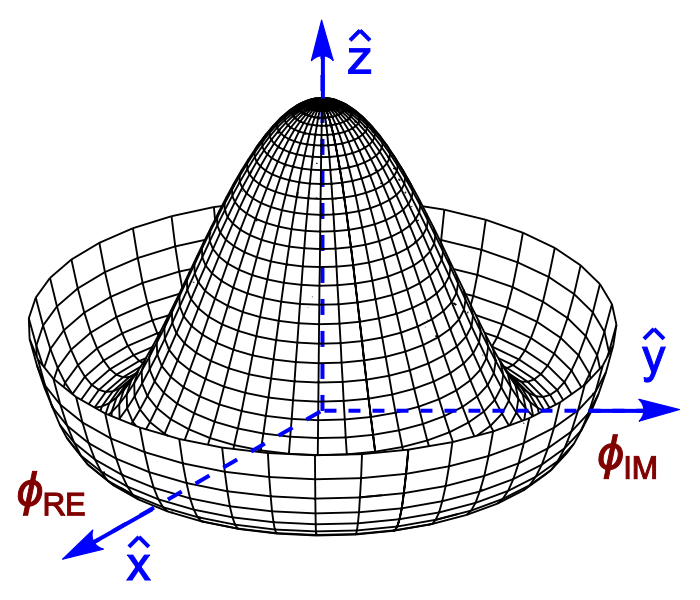
\includegraphics[width=0.5\textwidth]{Figures/theory/higgsPotential}
  \caption{Higgs `Mexican Hat' potential}
  \label{fig:MexHat}
  \end{center}
\end{figure}

The convention is to chose the \ac{VeV} as 
\begin{equation}
\langle 0 | \Phi | 0 \rangle = \left(  
\begin{array}{c}
0 \\
v/\sqrt{2}
\end{array} \right)
\text{ where }
v = \sqrt{\frac{- \mu^{2}}{\lambda}}
\end{equation}
as the minimum of the Higgs potential, given by $\Phi^{\dag} \Phi = \frac{1}{2} (- \mu)^{2}/\lambda$, 
is chosen to be consistent with the ground state of the vacuum.
Fluctuations from this zero point are then parametrized in terms of the four real scalar fields $\theta_{1} , \theta_{2} ,\theta_{3},$ and $h(x)$.
%
\begin{equation}
\Phi(x) = \left(  
\begin{array}{c}
\theta_{2} + i \theta_{1} \\
v/ \sqrt{2} + h(x)/ \sqrt{2} - i \theta_{3}
\end{array} \right)
= e^{i \tau \cdot \theta(x)/v}
 \left(  
 \begin{array}{c}
 0 \\
 v/\sqrt{2} + h(x)/\sqrt{2} 
 \end{array} 
 \right)
\end{equation}
%
The four scalar fields can be interpreted as four massless Goldstone bosons.
The exponential factor is recognised as a $SU(2)$ gauge transformation, so by moving to a different gauge in which this term becomes unity (the unitary gauge), we can arrive at
\begin{equation}
\Phi(x)' = \frac{1}{\sqrt{2}}
 \left(  
 \begin{array}{c}
 0 \\
 v + h(x) 
 \end{array} 
 \right).
 \label{eq:unitaryGauge}
\end{equation}
Substituting this expression for $\Phi'(x) = \Phi(x)$ into the covariant derivative term of $\mathcal{L}_{H}$, using Eq.~\ref{eq:EWKcovariant}, 
the mass terms for the three gauge bosons we require to complete the electroweak unification present themselves:
\begin{equation}
(D_{\mu}\Phi)^{\dag}(D^{\mu}\Phi) = \frac{1}{2}(\partial_{\mu}h)^{2} + \frac{g_{2}^{2}v^{2}}{8}\left( W^{+}_{\mu}W^{+\mu} + W^{-}_{\mu}W^-{\mu} \right)+ \frac{(g_{1}^{2}+g_{2}^{2})v^{2}}{8}Z_{\mu}Z^{\mu} + 0 A_{\mu}A^{\mu}.
\label{eq:covariantWithHiggsMech}
\end{equation}
Here, we have substituted in the physical gauge bosons $W^{\pm}_{\mu}, Z_{\mu}$ and $A_{\mu}$ for the fields $W^{i}_{\mu}$ and $B_{\mu}$.
This mechanism for spontaneous symmetry breaking gives the expected mass terms of the form $\frac{1}{2}m^{2}X_{\mu}X^{\mu}$ for the $W^{\pm}$ and $Z$ in terms of their couplings:
%
\begin{eqnarray}
m_{W} &=& \frac{g_{2}v}{2}\\
m_{Z} &=& \frac{\sqrt{g_{1}^{2} + g_{2}^{2}} \hspace{0.2em} v}{2} = \frac{m_{W} }{\cos \theta_{W} }.
\end{eqnarray}
% 
Crucially, the photon remains massless. 
By moving to the unitary gauge, we have lost three of the Goldstone bosons, 
or equivalently three degrees of freedom.
The fourth massless Goldstone boson has become a massive scalar boson, the \ac{SM} Higgs boson, with mass $m_{H} = \sqrt{-2\mu^{2}}$. 
The three lost degrees of freedom correspond to the longitudinal polarizations of the new massive boson.

Adding the Higgs potential to the \ac{SM} Lagrangian has allowed massive gauge bosons in a gauge invariant way. 
The remaining missing fermion mass terms can now be filled in using a similar method. 
By adding a Yukawa coupling (that is invariant under $SU(2)$) between the Higgs field and the fermions in the Lagrangian, 
the same Higgs boson can generate their masses.
The additional terms in the Lagrangian are of the form
\begin{equation}
\mathcal{L}_{Yukawa} =  k_{e} \bar{L} \Phi e_{R} + h.c. +  
 \left( k_{u} \bar{Q_{L}} \Phi d_{R} + k_{d} \bar{Q_{L}} \tilde{\Phi} u_{R} \right) + h.c
\end{equation}
where $\tilde{\Phi} = i \tau_{2} \Phi^{*}$ for up-type quark wavefunctions is necessary for gauge invariance. 
In the same unitary gauge of Eq.~\ref{eq:unitaryGauge}, we find
the couplings of the fermions to the Higgs field are then equal to their masses; 
$m_{e} = k_{e} v / \sqrt{2}$ and similarly for $m_{u}, m_{d}$ where $k_{u}$ and $k_{d}$ are arbitrary, non-diagonal $3\times3$ matrices.
These are the \ac{CKM} matrices and dictate the flavour structure of the \ac{SM}~\cite{Cabibbo,Kobayashi01021973}. 


The remaining piece of the \ac{SM} not mentioned above is the description of the strong interaction. 
It only affects coloured particles, and as a result of its $SU(3)$ gauge invariance, 
the generators are the Gell-Mann matrices $\lambda_{a}$ where $a = 1,2,...8$ which give rise to eight gluons $G_{a}$. 
To incorporate the strong force, which gives rise to \ac{QCD}, we simply add the $SU(3)$ terms to the covariant derivative and $\mathcal{L}_{kin}$:
\begin{equation}
D_{\mu} &= \partial_{\mu} - i g_{1} \frac{Y}{2} B_{\mu} - ig_{2} \frac{\tau_{i}}{2} W^{i}_{\mu} - ig_{3} \frac{\lambda_{a}}{2} G^{a}_{\mu} \\
\frac{1}{4}F_{\mu \nu}F^{\mu \nu} &= \frac{1}{4}\left( B_{\mu\nu}B^{\mu\nu} +  W_{\mu\nu} W^{\mu\nu} +  G^{a}_{\mu\nu} G^{\mu\nu}_{a} \right).
\label{eq:covariantDeriv}
\end{equation}

Gauge invariance dictates the form of the electroweak Lagrangian. 
Spontaneous symmetry breaking via the Higgs mechanism leads to three to massive gauge bosons, one massless gauge boson, and one massive scalar boson.
The \ac{SM} Lagrangian can then be written by summing the various terms discussed above:
\begin{equation}
\mathcal{L}&=\mathcal{L}_{int}+\mathcal{L}_{kin}+\mathcal{L}_{H}+\mathcal{L}_{Yukawa} \\
		  &= \bar{\psi} i \gamma^{\mu} D_{\mu} \psi - \frac{1}{4}F_{\mu \nu}F^{\mu \nu} + |D_{\mu}\Phi|^{2} + \mu^{2} |\Phi|^{2} - \lambda |\Phi|^{4} +  \left( \bar{\psi_{i}} k_{ij} \psi_{j} + h.c \right)  
\label{eq:SMlagrangian}
\end{equation}
%


\section{Motivation for Physics Beyond the Standard Model \label{th:BSM}}
%
Despite its many successes, fundamental theoretical flaws in the \ac{SM}, 
as well as observed phenomena it fails to explain, imply there must be new physics at some energy scale. 
Various experimental observations -- gravity, the matter-antimatter imbalance in the universe, neutrino oscillations, dark matter -- all have no explanation in the \ac{SM}.
Questions of the naturalness of the theory with regard to fine tuning the mass of the Higgs boson, the non-unification of the fundamental forces, and the seemingly arbitrary number of parameters lead many theorists to believe
the \ac{SM} to be a low energy approximation of some new form of physics -- 
physics which solves the underlying theoretical problems,
as well as filling in the `holes'.

Gravity has no place within the \ac{SM}; there is no interaction to explain the gravitational attraction felt by the fundamental particles which is so evident at large distance scales. 
Despite its negligible influence on subatomic particles at the energy scales probed by the \ac{LHC}, the gravitational force cannot be reconciled with a quantum theory.
%

In addition, there is insufficient \ac{CP} violation within the \ac{SM} to explain the observed matter dominance in the Universe. 
The \ac{CP} violation in the kaon and $D_{0}$ meson sectors is not enough to explain why only matter remains from the Big Bang, 
in which matter and antimatter are thought to have been produced in even quantities. 
Physics \ac{BSM} is necessary to introduce another source of it in order to explain we why are here at all; why all matter did not annihilate soon after it was created.

%

The solar neutrino problem, in which there were far less $\nu_{e}$ arriving at the Earth from the Sun than solar models predicted, 
was solved with the discovery of neutrino oscillations~\cite{SolarNeut}. 
The $\nu_{e}$, on their flight from the sun, were changing state so that when they were measured on Earth they were no longer in the electron-like weak eigenstate. They had oscillated into a different weak eigenstate, and so appeared to have disappeared when measured in electron-like charged current interactions. 
Neutrino oscillations imply that there is a mass difference between the different mass eigenstates of the neutrinos, $\nu_{1}, \nu_{2}, \nu_{3}$, which are a superposition of their weak flavour eigenstates $\nu_{e}, \nu_{\mu}, \nu_{\tau}$.
A mass difference means each type of neutrino must have a mass (albeit small) -- in contradiction of the massless, left handed neutrinos present in the \ac{SM}.
New physics is needed to explain massive neutrinos.


The flaw in the \ac{SM} getting perhaps the most attention at the moment, in the current post-Higgs boson discovery era, is that it has no candidate for \ac{DM}. 
Astronomical observations of galaxy rotation curves~\cite{GalRotCurves}, gravitational lensing~\cite{GravLensing1,GravLensing2}, the \ac{CMB}~\cite{Planck2013}, the Bullet Cluster~\cite{bulletCluster}, and large scale structures~\cite{LargeScaleStructuresDM} imply that there is a `dark' matter present in the universe; 
dark because it does not interact with electromagnetic radiation. 
Its presence is only inferred by its gravity. 
Therefore it must be also stable and weakly interacting -- we have found no unequivocal evidence of \ac{DM} decay products (although recent gamma-line spectra from the centre of the galaxy could suggest \ac{DM} annihilation~\cite{FermiDMgamma} ). 
Astronomical observations imply that \ac{DM} makes up around 26.8\% of the energy budget of the universe, compared to the 4.9\% of the matter the \ac{SM} is comprised of. 
For our model of the fundamental forces and particles of the universe, the \ac{SM}, 
to have no \ac{DM} candidate leads us to question it -- 
and come to the conclusion there must be something more.
It is perhaps worth mentioning that Dark Energy, 
which is theorized to constitute the remaining 68.3\% of the energy budget, 
and is responsible for the observed expansion of the universe, is not understood at all!


While the above are pieces of experimental evidence that cannot be explained by the \ac{SM}, 
there are also theoretical problems with the model when calculating the radiative corrections to the Higgs boson mass.
We saw in Eq.~\ref{eq:HiggsPot} that the scalar potential giving rise to the Higgs Boson $h$ is of the form
\begin{equation}
V \sim m_{H0}^{2} h^{2} + \lambda h^{4}.
\end{equation}
The presence of the quartic term, proportional to $\lambda$, implies the Higgs interacts with itself at loop level. 
This self-interaction adds another, quadratically divergent term to the mass of the Higgs, $m_{H}$:
\begin{equation}
m_{H}^{2} \sim m_{H0}^{2} + \frac{\lambda}{4 \pi ^{2}} \Lambda^{2} + \delta M_{H}^{2},
\label{oneloopHiggsMass}
\end{equation}
where $\Lambda$ is some cut-off energy scale to where the physics is valid.
If there is no new physics between the electroweak scale at $\sim 100~\GeV$ and the Planck scale, then $\Lambda$ is of the same order as the Planck scale.
Indirect constraints on the Higgs mass from measurements of the $\W$ and top quark masses~\cite{higgsMassConstraint1,higgsMassConstraint2} imply that the Higgs mass is around the electroweak scale, and indeed direct measurements of the Higgs boson mass are around 125~\GeV~\cite{HiggsLegacyCMS,HiggsLegacyATLAS} -- not $M_{Pl}$.
The term $\delta M_{H}^{2}$ then must cancel out the term in $\Lambda$; ie there must be a cancellation of order $M_{Pl} \sim 10^{18}$.
To put this hierarchy problem another way, there is a precise fine-tuning necessary, of one part in $10^{18}$.
Although possible, this is very unnatural, and drives the much of the theoretical motivation for \ac{BSM} physics.



\ac{SUSY}~\cite{susyMot1,susyMot2} is one example of an extension to the \ac{SM} which can solve many of its problems, and is the subject of remainder of this chapter, as well as the analysis work done in this thesis. 
It is probably the most popular and well studied \ac{BSM} theory in the community, however is not alone: models of
Large Extra Dimensions~\cite{ADDextraDimensions}, the 
SeeSaw Mechanism~\cite{seesawMech1,seesawMech2}, and
Little Higgs~\cite{LittleHiggsRev}
are just a few examples of many theories which attempt to explain the shortcomings of the \ac{SM} by introducing new physics.



\section{Supersymmetry \label{th:SUSY}}

\ac{SUSY} first emerged in the 1970's as a result of the mathematical considerations of \ac{QFT}. 
The Coleman-Mandula theorem~\cite{ColemanMandula}, 
which states that space time and internal symmetries cannot be combined anything but trivially, 
was found to have a hole in it~\cite{Gol’fand_Likhtman_1971}. 
This allows a symmetry between fermions (f) and bosons (b):
\begin{equation}
\hat{O} | f \rangle = |b \rangle ; \hspace{2em}  \hat{O} | b \rangle = |f \rangle 
\label{fermionbosonTrans}
\end{equation}
where $\hat{O}$ is the supersymmetric operator generating the transition.
\ac{SUSY} relates particles of different spin, where they differ by a half integer unit,
and the Lagrangian remains invariant under transformations such as those in Eq.~\ref{fermionbosonTrans}.
The generated particles, or sparticles, have the all of the same quantum numbers as those particles they have been generated with (but for the spin) -- so they have the same mass. 

If we reconsider the one loop corrections to the Higgs field, h, 
with massive fermions \psi and massive scalars \phi~\cite{susyandsuch} (which can be generated by a supersymmetric transition as they differ in spin by a half-integer unit), we see additional terms in $m_{H}^{2}$:
\begin{equation}
\begin{split}
m_{H}^{2} \sim m_{H0}^{2} &+ \frac{\lambda_{F}^{2}}{4 \pi ^{2}} (\Lambda^{2} + m_{F}^{2})  - \frac{\lambda_{S}^{2}}{4 \pi ^{2}} (\Lambda^{2} + m_{S}^{2}) \\
&+ \text{ logarithmic divergences } + \text{ uninteresting terms }.
\label{oneloopHiggsMassSUSYfermionScalar}
\end{split}
\end{equation}
Crucially, there is a relative minus sign between the two quadratic terms in $\Lambda$, a result of Fermi statistics.
If the couplings between the Higgs and the fermion $\lambda_{F}$ and scalar $\lambda_{S}$ are equal, then 
the quadratic terms in $\Lambda$ cancel, and all that remains of the troubling quadratic divergence of Eq.~\ref{oneloopHiggsMass} are the mass terms:
\begin{equation}
m_{H}^{2} \sim m_{H0}^{2} &+ \frac{\lambda_{F}^{2}}{4 \pi ^{2}} (m_{F}^{2} - m_{S}^{2}) .
\label{oneloopHiggsMassSUSYresolved}
\end{equation}
Here, the fermion and scalar have been generated by a supersymmetric transition, and thus have the same quantum numbers. 
They have the same mass -- and so the quadratic term completely cancels out.
The fine tuning problem has been solved.
However, no scalar particle has been observed with the same quantum numbers, and mass, of any fermion.
No scalar particle with the same quantum numbers and different mass have been observed either, up to the energies probed -- which, at the LHC, is of order 1~\TeV.

It was the theoretical breakthrough in the 1980's that allowed \ac{SUSY} to be a broken symmetry: 
the mathematical framework remains consistent even if the masses are not the same.
Then, the second term in Eq.~\ref{oneloopHiggsMassSUSYresolved} remains -- 
but, provided the masses are `not too different' 
(where the allowed differences are seemingly a matter of opinion, deemed `naturalness', but general consensus is of order a few \TeV so reachable at \ac{LHC} energies) 
- the issue of the fine-tuning of the Higgs mass is resolved, as the huge corrections necessary with no \ac{SUSY} are now far more manageable.

\ac{SUSY}, then, is a \ac{BSM} theory with a foundation in the mathematics of \ac{QFT}s, which, as a consequence of its symmetry, cancels out the huge quadratic divergences in the Higgs mass, making it very appealing. 
The \ac{SM} becomes a part of a wider supersymmetric model that maintains the same $SU(3)\times SU(2) \times U(1)$ gauge symmetry. 
In the \ac{MSSM}, every \ac{SM} particle gets a supersymmetric particle (sparticle) partner which has the same quantum numbers but differs a half integer unit in spin and has a greater mass. 
A rich sparticle phenomenology results, as the entire spectrum of \ac{SM} particles is doubled.
For example, the left-handed quark doublet gets a doublet of left handed scalars:
\begin{equation}
Q_{L} = \left(  
 \begin{array}{c}
 u \\
 d 
 \end{array} 
 \right)_{L}
 \hspace{1em}; \hspace{1em}
 \tilde{Q}_{L} = \left(  
 \begin{array}{c}
 \tilde{u}_{L} \\
 \tilde{d}_{L} 
 \end{array} 
 \right)
\end{equation}
and similarly, $L, e_{R}, u_{d}, d_{R}$ defined in Section~\ref{th:EW} get $\tilde{L}, \tilde{e}_{R}, \tilde{u}_{d}, \tilde{d}_{R}$ which are both contained in the respective $SU(2)_{L}$ or $U(1)$ superfields.
Additional superfields contain the \ac{SM} bosons and their fermionic partners: the gluons $g^{a}$ and gluinos $\tilde{g}^{a}$; the three weak bosons $W_{i}$ and the winos $\tilde{w}_{i}$; and the $U(1)$ boson $B$ß and its partner the bino $\tilde{b}$. 
To cancel out gauge anomalies, the \ac{SM} $SU(2)_{L}$ Higgs doublet of scalars becomes two doublets $H_{u}$ and $H_{d}$, which then require two Higgs doublets of fermions for the higgsinos $\tilde{h}$. 


\subsection{R Parity and Dark Matter\label{th:RParity}}
The full \ac{MSSM} Lagrangian can be found elsewhere~\cite{susyandsuch}. 
Suffice to say, there are terms which permit lepton and baryon number violating interactions that can mediate proton decay, and give rise to interactions such as the one in Fig.~\ref{fig:pdecay}.
\begin{figure}[htbp]
  \begin{center}
  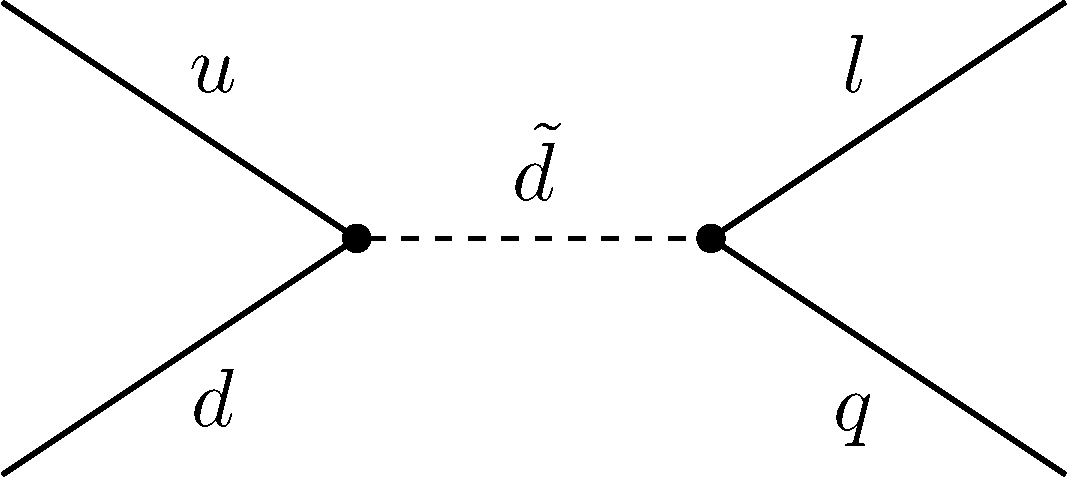
\includegraphics[width=0.4\textwidth]{Figures/theory/RPVpdecay}
  \caption{Example of a lepton and baryon number interaction which would mediate proton decay.}
  \label{fig:pdecay}
  \end{center}
\end{figure}
There are very stringent limits on proton decay; $\tau > 10^{33}$ years~\cite{PDG}, so interactions such as these must be highly suppressed, if allowed at all. 
The class of \ac{SUSY} models which do not permit lepton and baryon violating interactions have an additional symmetry in R parity, which is defined as
\begin{equation}
R = (-1)^{3(B-L)+s},
\end{equation}
where $B$ is the baryon number, $L$ the lepton number, and $s$ the spin of the particle.
A consequence of R parity conserving \ac{SUSY} is that sparticles are always produced in pairs, and any sparticle decay will always result in another sparticle being produced.
So any \ac{SUSY} decay chain, as well as producing many \ac{SM} particles, will always result in a single sparticle -- the lightest of the \ac{SUSY} spectra, so cannot decay further.
This is then the \ac{LSP}, and must be stable.
Cosmological bounds on light charged or coloured stable particles~\cite{PDG} imply the \ac{LSP} (if it exists) must be neutral.
A stable, neutral, weakly interacting \ac{LSP}, key to the popularity of \ac{SUSY}, then very naturally gives a \ac{DM} candidate.
The \ac{LSP}, with a collider signature much like a neutrino, will exit a detector having deposited no energy as it interacts with none of its material.
There will instead be an imbalance in momentum, leading to a missing transverse energy signature.

\subsection{Unifying the forces}

Another feature of \ac{SUSY} which makes it very popular with the theory community 
is the natural unification of the weak, electromagnetic and strong forces at the \ac{GUT} scale.
The strengths of each of these forces change with distance, or equivalently energy -- their coupling constants `run'. 
At very small distances, or very high energies, such as those at the time of the Big Bang, masses of any particles involved are completely negligible, and the strengths of interactions can be investigated.
With the vanilla \ac{SM} of Section~\ref{th:sm}, there is not a single point where the three coupling constants unite, or become one, unified interaction. 
However, when \ac{SUSY} is added in, all three forces become unified at a single point around $10^{16}$~\GeV~\cite{GUT}, see Fig.~\ref{fig:SUSgut}.

\begin{figure}[htbp]
  \begin{center}
  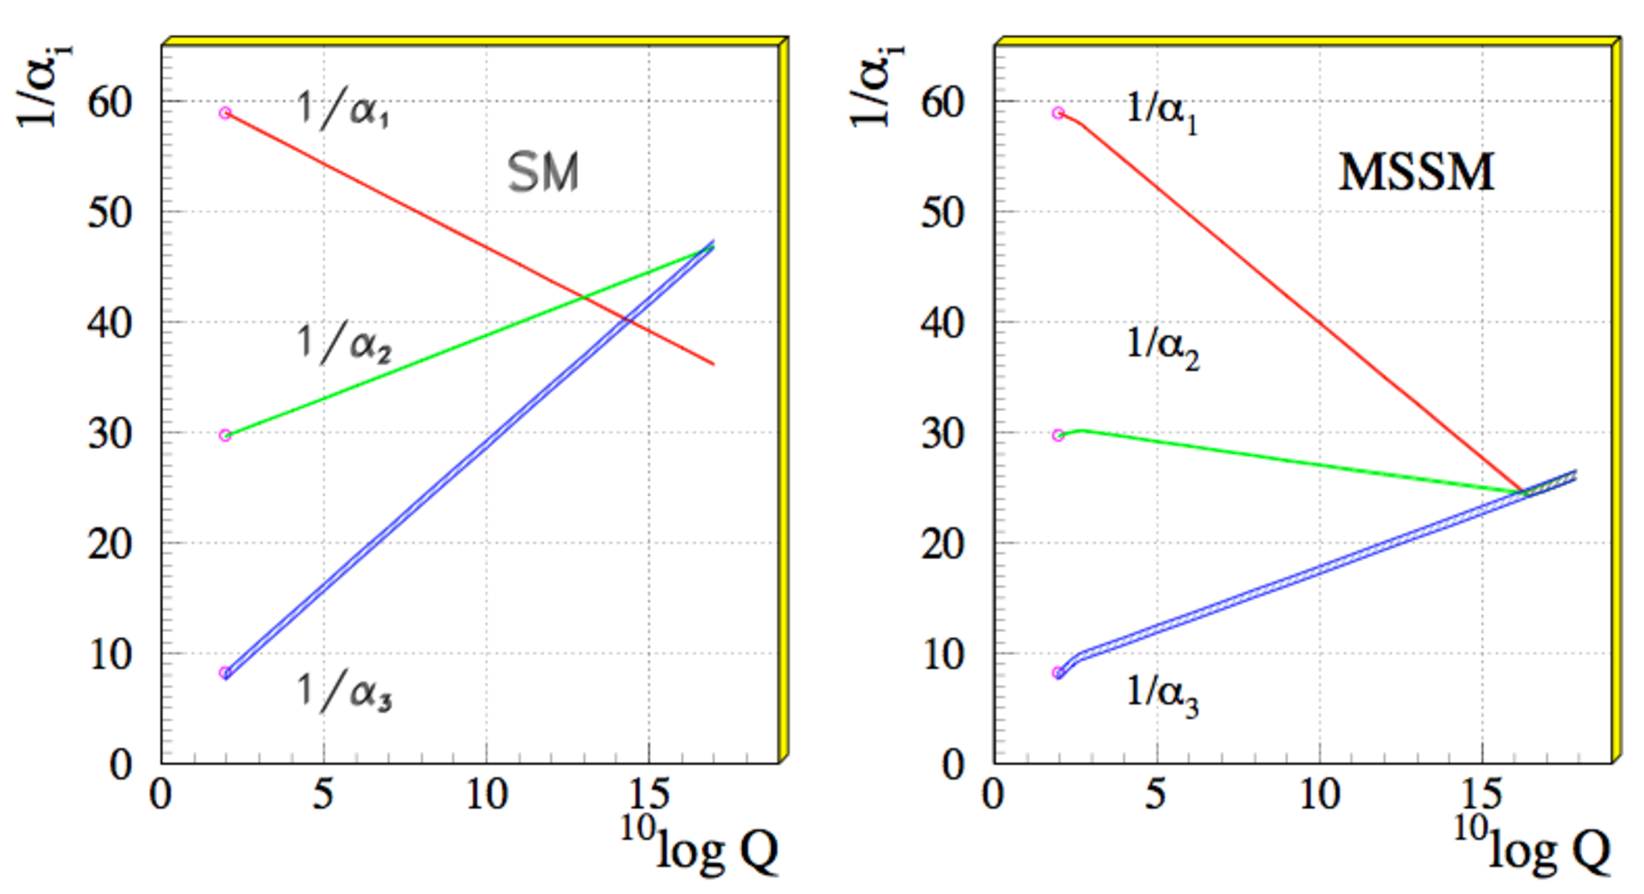
\includegraphics[width=0.8\textwidth]{Figures/theory/GUTunification}
  \caption{The running coupling constants of the electromagnetic, strong and weak forces with increasing energy or decreasing distance. Once \ac{SUSY} has been added in, the three unify around $10^{16}$~\GeV, hinting at a \ac{GUT}. Taken from ~\cite{GUTpic}.}
  \label{fig:SUSgut}
  \end{center}
\end{figure}

This very elegant picture of the early universe is very attractive: one single force dominated while the energy density was high enough, and then later, a transition occurred when the three forces became distinct.
The idea of a \ac{GUT}, with some higher symmetry group, that can dictate all of the behaviour we observe in the universe is very appealing to theorists.


\subsection{Breaking Supersymmetry and Naturalness \label{th:susyBreaking}}

We have mentioned that \ac{SUSY} is a broken symmetry if it exists in nature.
The possible mechanism of the spontaneous symmetry breaking is beyond the scope of this thesis, 
but different \ac{SUSY} breaking mechanisms lead to many different sparticle phenomenologies~\cite{susyMot2}. 
It is usually assumed that the \ac{SUSY} breaking occurs at some high scale $\sim M_{Pl}$, and that it is ``soft''~\cite{softsusy}, which leads to logarithmic, rather than quadratic divergences.
The correction to the Higgs mass then takes the form
\begin{equation}
\delta m_{H}^{2} \sim \left( m_{\tilde{q}}^{2} - m_{q}^{2} \right) \log{\Lambda}.
\end{equation}
The largest contribution to $\delta m_{H}$ is from the top quark, 
because it is so much more massive than all other \ac{SM} fermions at 173~\GeV.
To keep $\delta m_{H}$ reasonably small, and the fine tuning issue minimal, the supersymmetric partner to the top quark, the top squark \sTop should be fairly close in mass to 173~\GeV.
Figure~\ref{fig:SUSYmot} shows the correction to the Higgs mass due to the top quark loop, and the corresponding loop correction from the top squark, which acts to cancel the divergence in the Higgs mass out.

\begin{figure}[htbp]
  \begin{center}
  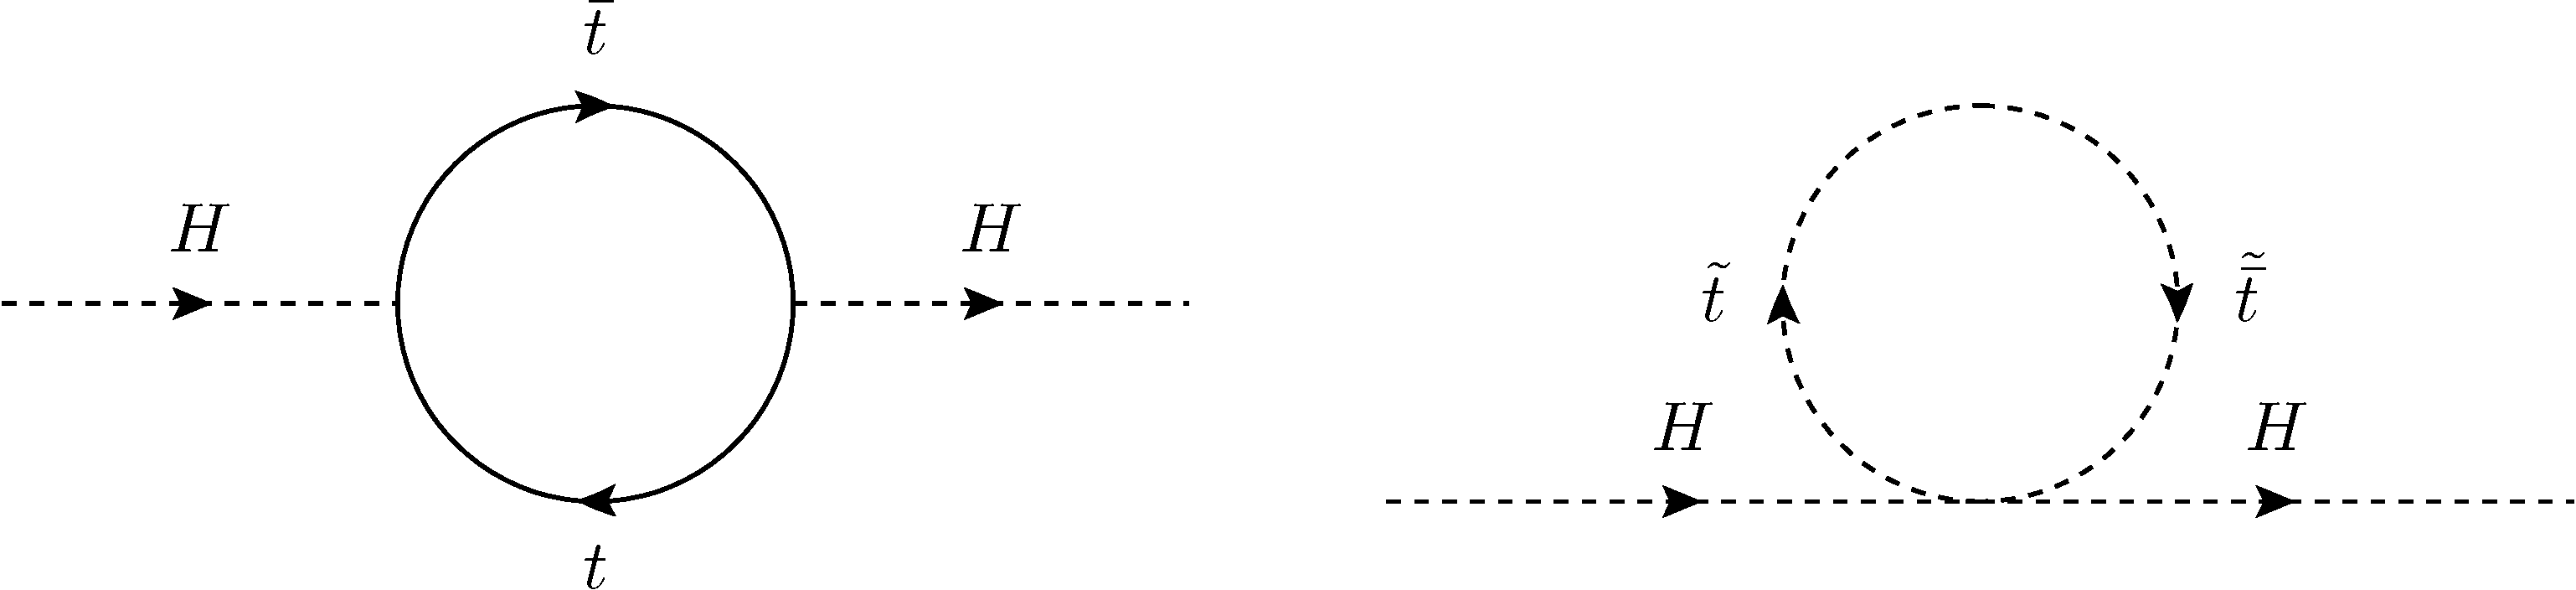
\includegraphics[width=0.8\textwidth]{Figures/theory/SUSYmot}
  \caption{The loop contributing to the Higgs mass due to the top quark, left, and the cancellation of the loop due to the top squark, right.}
  \label{fig:SUSYmot}
  \end{center}
\end{figure}

Such naturalness arguments motivate a light \sTop, and a bottom-up approach to any \ac{SUSY} spectrum.
The biggest Yukawa couplings come from the heaviest \ac{SM} particles, i.e. the third generation.  
To keep corrections to the Higgs mass small, the third \ac{SUSY} generation is expected to be the lightest, 
and in reach of the \ac{LHC}~\cite{natSUSY3,natSUSY4}.
First generation squarks and sleptons can be much heavier, even up at the Plank scale, 
while keeping a natural \ac{SUSY}.

\subsection{Searching for Supersymmetry at Colliders}
\label{sec:susycolliders}

Having motivated \ac{SUSY} as a extension of the \ac{SM} which has the potential to very nicely solve the hierarchy problem, give us a \ac{DM} candidate and unify the three fundamental forces at the \ac{GUT} scale, we ask ourselves how best to search for any possible signs of it at a collider.
In R parity conserving \ac{SUSY}, the \ac{LSP} exits the detector leaving nothing but an imbalance of momentum; at hadron colliders, this imbalance is evident in the transverse plane as \MET.
In addition, typical \ac{SUSY} decay chains have multiple legs, as a heavy sparticle produced in the pp collision decays down the \ac{SUSY} spectrum. 
A \ac{SM} particle (which may itself decay) is emitted at each step until the energy is small enough that only the \ac{LSP} can be emitted, along with a final \ac{SM} particle.
Each event has two such decay chains as the original sparticle is pair produced. 
The array of decays possible, as well as the energies involved, depend entirely on the \ac{SUSY} spectrum considered, which in turn is dependent on the type of \ac{SUSY} breaking.
An example of this kind of \ac{SUSY} decay chain is shown in Fig.~\ref{fig:SUSYdecaychain}. 
Here, the LSP is shown as \chiOneZero. 
Such $\tilde{\chi}^{0}$ states are a neutral superposition of higgsino, wino and bino states; the exact composition is again \ac{SUSY} model dependent.
Charged superpositions are written as $\tilde{\chi}^{\pm}$ and often feature in such decay chains.

\begin{figure}[htbp]
  \begin{center}
  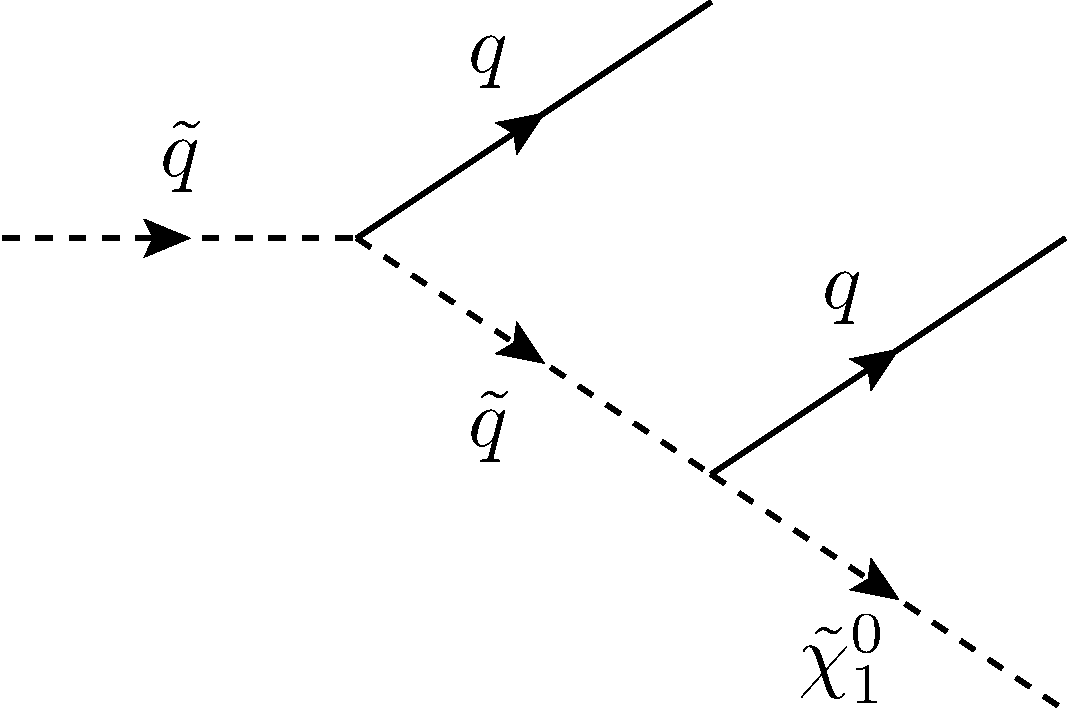
\includegraphics[width=0.4\textwidth]{Figures/theory/susyDecayChain.pdf}
  \caption{Example of a \ac{SUSY} decay chain, in which there are several quarks emitted as well as the \ac{LSP}. Two of these decay chains will be present in each event due to the pair production of the parent \squark.}
   \label{fig:SUSYdecaychain}
   \end{center}
\end{figure}


To be sensitive to these \ac{SUSY} signatures, which have high particle multiplicity and lots of energy in the final state, traditional searches have revolved around looking for multiple final state objects, plus a significant amount of \MET.
To be as model independent as possible, searches are generic.
There are searches for multijet events (arising from a decay chain similar to that in Fig.~\ref{fig:SUSYdecaychain}), 
same or opposite sign dilepton events, multi-lepton events, 
events which have both leptons and jets, or photons,
jets which are tagged as arising from a b-quark, 
events with lots of hadronic energy deposited ($H_{T}$): see Refs.~\cite{CMSdilepbjets,CMSmultijet1,CMSmultijet2,CMSsinlepJets,CMSmultilep,CMSsinglelep,CMSdiphotonH,CMSHZbosons,CMSleptonsWZH}.
Innovative methods of controlling the large backgrounds, particularly as a result of \ac{QCD} multijet events, have been developed~\cite{CMSrazor7TeV,CMSalphaT,CMSmt2}.

Stringent bounds were placed on the \ac{CMSSM} during the first \ac{LHC} run~\cite{constrainedCMSSM,finetuningcmssm}. 
It is a popular \ac{SUSY} model which simply reduces the multitude of free parameters in the \ac{MSSM} down to 5 by setting many of the masses to be equal. 
All scalar masses become $m_{0}$, all gaugino masses $m_{1/2}$, trilinear coupling are set to $A_{0}$, and the ratio of the \ac{VeV} of the two Higgs doublets is $\tan{\beta}$. 
The fifth parameter is the sign of $\tan{\beta}$.
Traditionally, searches are interpreted using the \ac{CMSSM} as it produces a simple phenomenology, enabling mass scans in four dimensions (plus a sign) rather than over one hundred in the full \ac{MSSM}. 
The phenomenology is also `easily' discoverable: parameters are fixed at the \ac{GUT} scale and extrapolated down to the electroweak scale (for example, the \Z pole mass), making mass differences between particles relatively large and so decay products reasonably energetic. 
Limits from searches using the CMS detector are shown in Fig.~\ref{fig:cmssmlimits}.
The lack of any sign of \ac{SUSY} in these direct searches, as well as limits from indirect searches sensitive to the parameters of the \ac{CMSSM} (such as $B_{S}\rightarrow \mu\mu$~\cite{BSmumuCombo}) have lead the community pursue less specific, alternative scenarios.


% %{\color{red} Should I put the summary plots here?}
 \begin{figure}[htbp]
   \begin{center}
   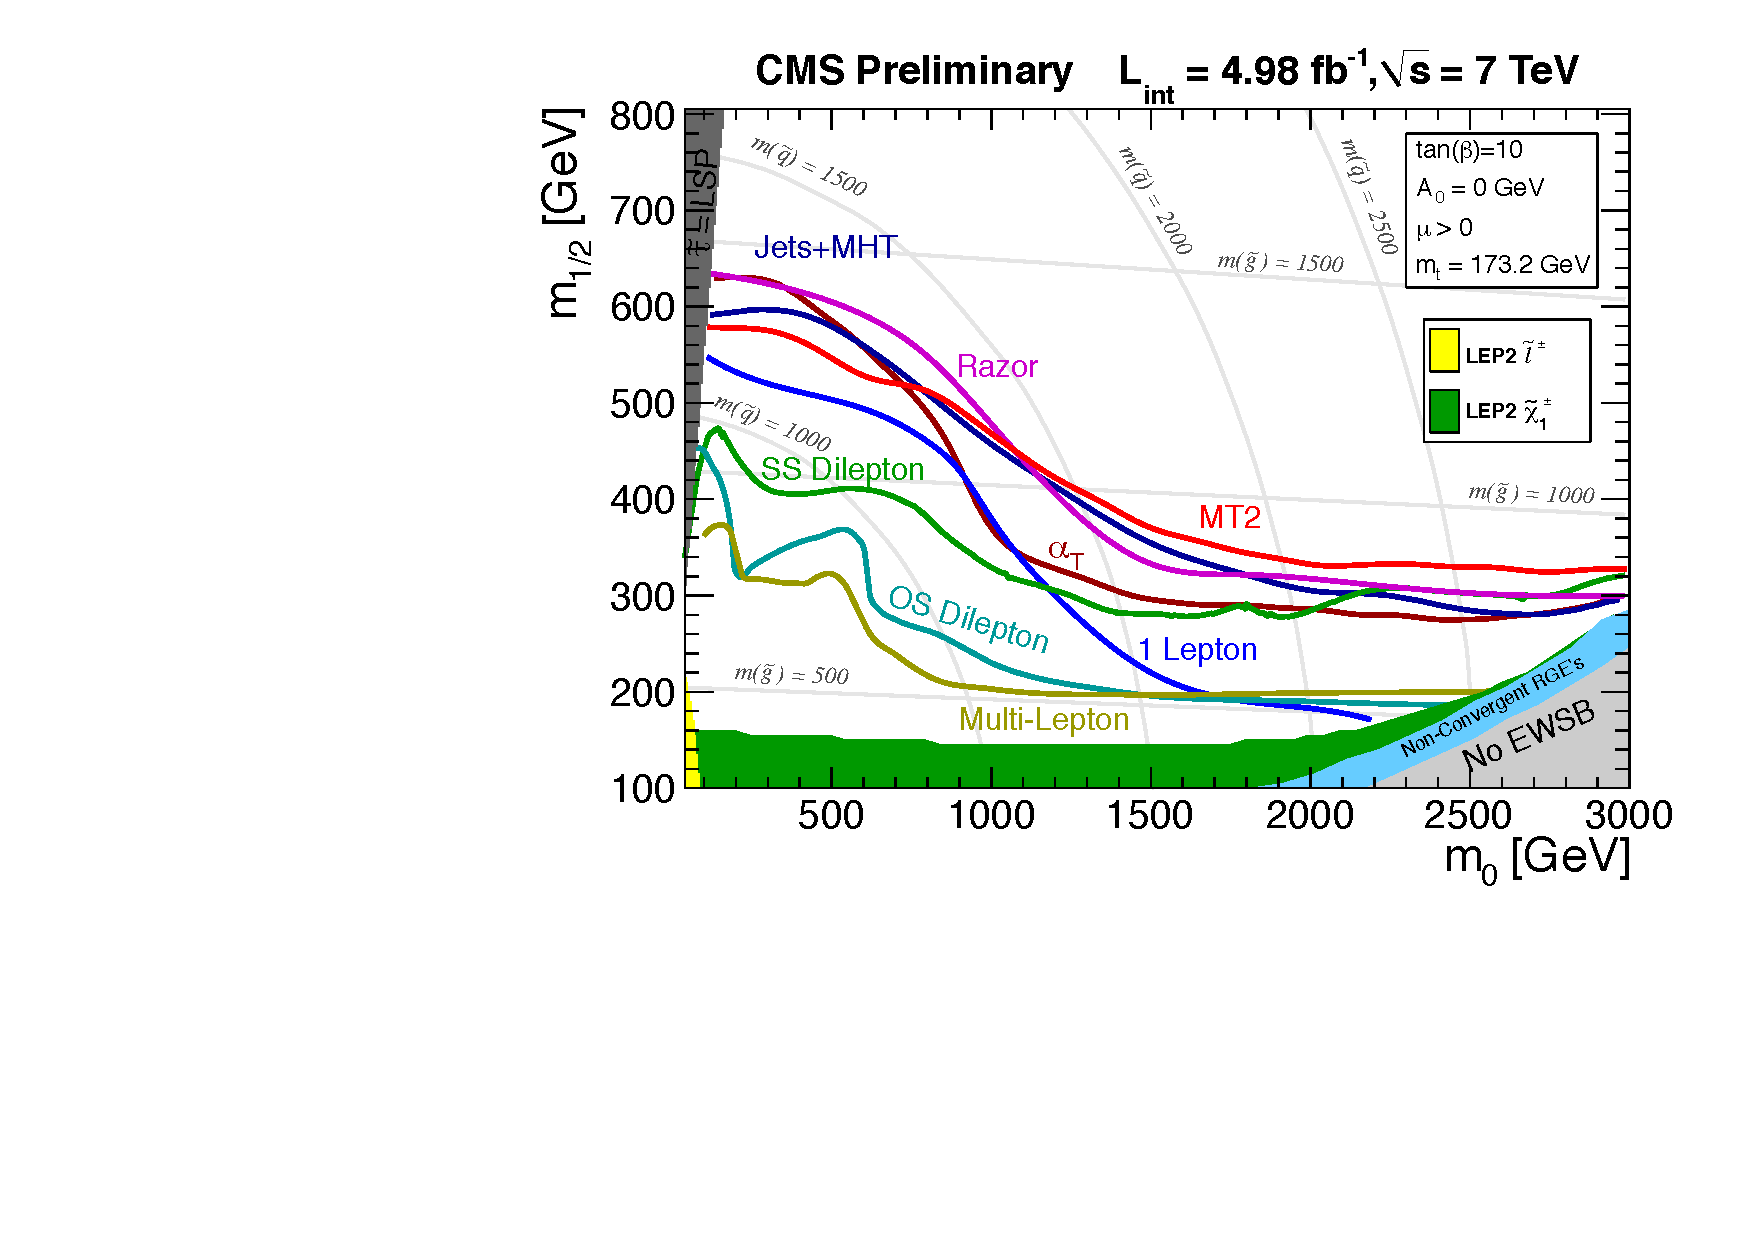
\includegraphics[width=0.7\textwidth]{Figures/theory/CMS_SUSY_2011Limits5fb_tanb10.pdf}
   \caption{The limits on the $m_{1/2}, m_{0}$ \ac{CMSSM} mass plane from \ac{CMS} with the full 7~\TeV dataset, taken from~\cite{tw:CMSSMlimits7TeV}.}
   \label{fig:cmssmlimits}
   \end{center}
 \end{figure}

A more model independent approach has been adopted more recently, with the use of \ac{SMS}~\cite{SMS1,SMS2,SMS3, SMSPaper}, which allow searches to be interpreted in the mass planes of various sparticles: in the mass of the \sTop, \sbottom, \squark and \chiOneZero for example.
All other sparticles than those probed are assumed to be very heavy and are integrated out.
%\ac{SMS} are discussed further in Section~\ref{sec:SMS}.

\begin{figure}[htbp]
  \begin{center}
  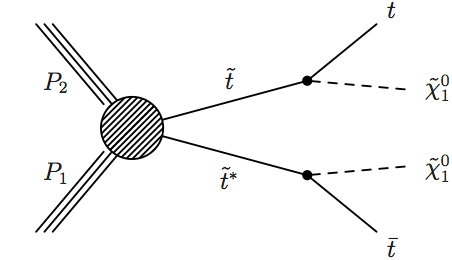
\includegraphics[width=0.5\textwidth]{Figures/theory/T2tt.png}
  \caption{An example of a \ac{SUSY} decay of the top squark. This is one of the simplified models probed by \ac{CMS} at the \ac{LHC}.}
  \label{fig:t2tt}
  \end{center}
\end{figure}


Figure~\ref{fig:t2tt} shows an example Feynman diagram for a particular decay of the \sTop, 
one of the \ac{SMS} hypotheses probed, 
which dominates if the top squark is heavy enough to produce an on-shell top quark when it decays.
Other decays dominate when this is not true, which can then be targeted with searches that have different kinematics than that of Fig.~\ref{fig:t2tt}: this will be the subject of Chapter~\ref{chap:sus13009}.
Such generic searches can also be simply applied to other models of \ac{BSM} physics.


At 7 and 8~\TeV, no evidence for \ac{SUSY} has been found at the \ac{LHC};
exclusion limits on squarks and gluinos are around 1~\TeV at 95\% \ac{CL}.
Searches have ruled out huge swathes of phase space, see Fig.~\ref{fig:cmssmlimits} and Fig.~\ref{fig:susy2013stop} that show the limits on the \ac{CMSSM} and the combined \ac{CMS} results on the \sTop, \chiOneZero mass plane at SUSY 2013 respectively.

\begin{figure}[t!]
  \begin{center}
  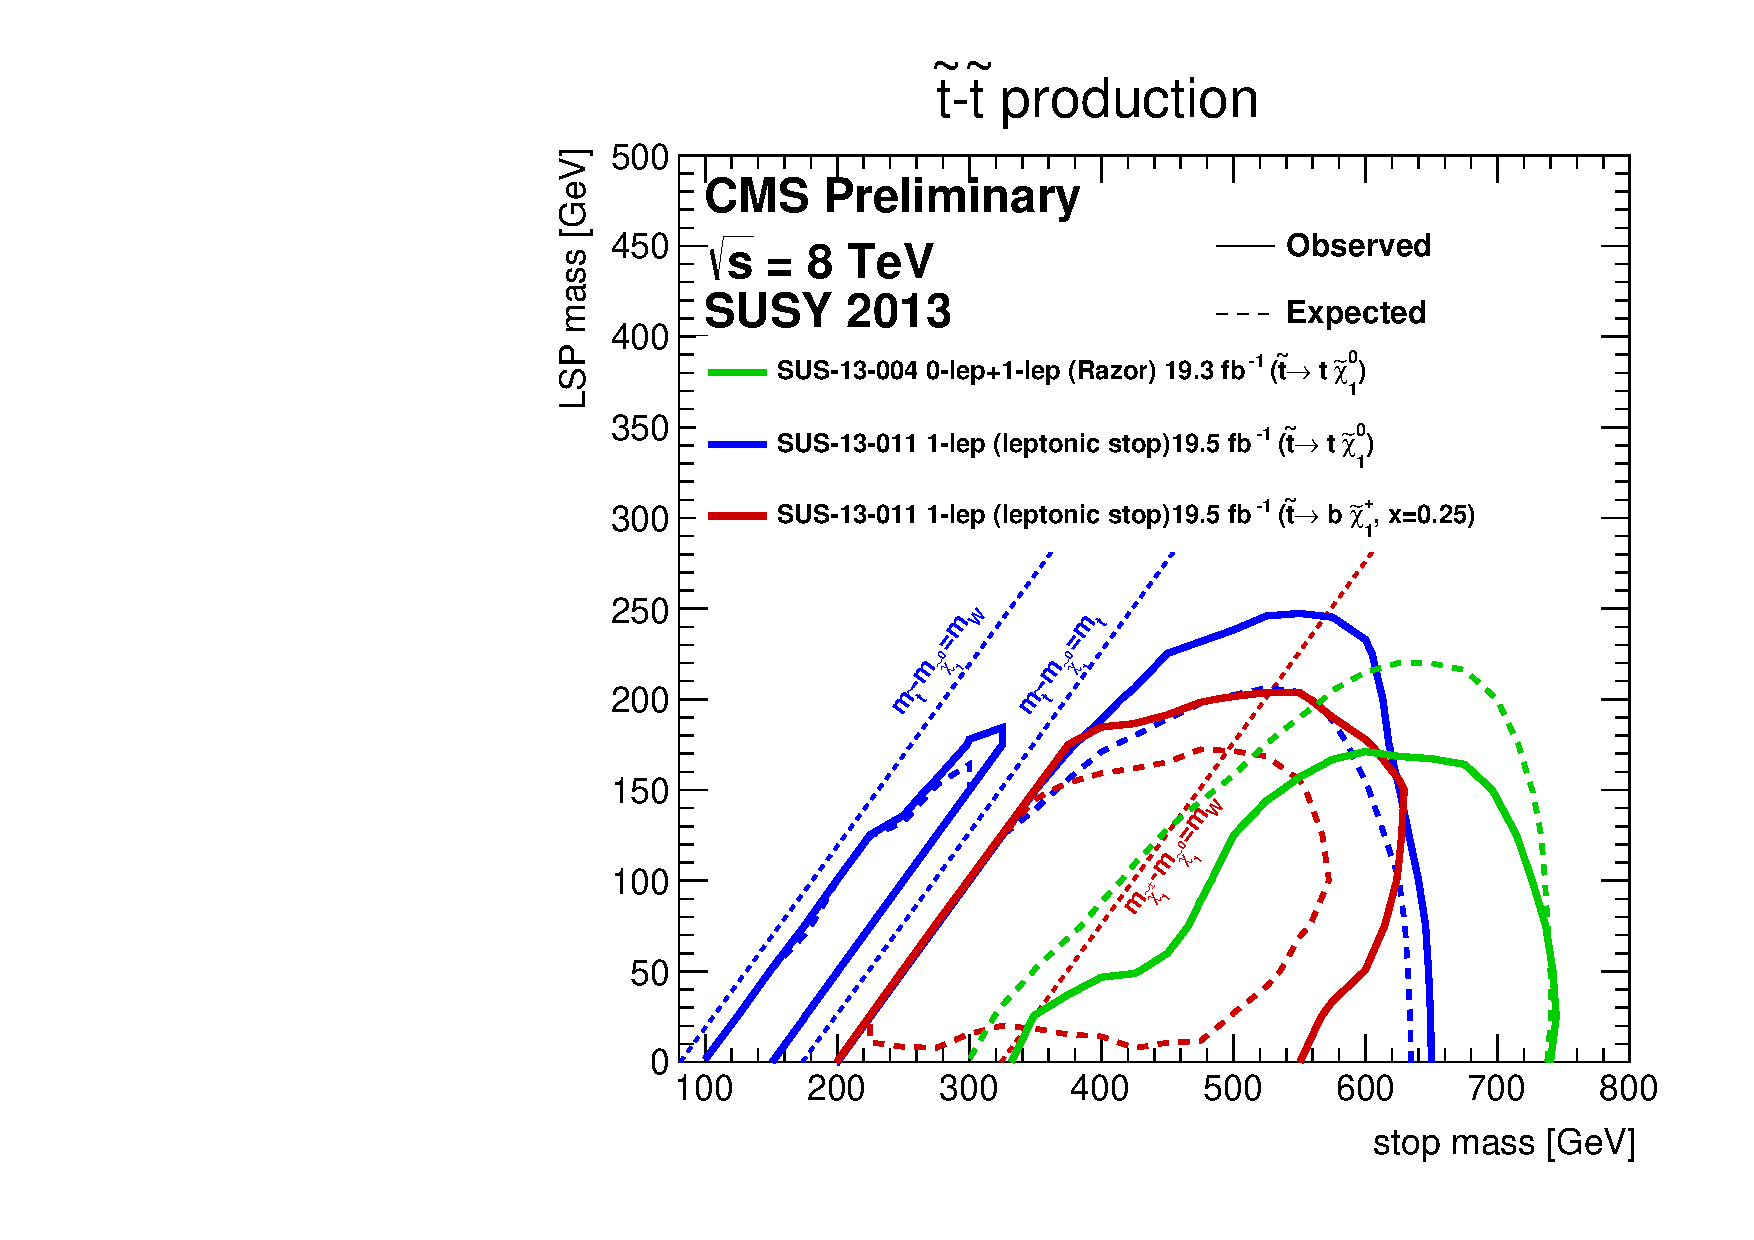
\includegraphics[width=0.7\textwidth]{Figures/theory/SUSY2013T2ttT6.pdf}
  \caption{The limits on the \sTop, \chiOneZero mass plane from \ac{CMS} at SUSY 2013~\cite{tw:SUSY2013T2tt}.}
  \label{fig:susy2013stop}
  \end{center}
\end{figure}


If~\ac{SUSY} is to persist as a convincing~\ac{BSM} theory, 
naturalness arguments in conjunction with a Higgs mass of $\sim 125$~\GeV imply that the third generation squarks should be light~\cite{natSUSYhiggs}.
Either \ac{SUSY} does not exist in a natural way and doesn't solve the theoretical problems in the \ac{SM} that it has been proclaimed to, it is just out of reach at the 8~\TeV \ac{LHC}, or \ac{SUSY} is somehow hidden.
Fig.~\ref{fig:susy2013stop} has areas which are not covered by the exclusion regions, 
where it has been suggested that \ac{SUSY} may be `hiding'. 
Traditional searches loose sensitivity in these regions.
For example, in the strip close to the kinematic limit, 
when the parent sparticle -- $m_{\sTop}$ in this case -- is close in mass to $m_{\chiOneZero}$,
decay products become very soft, so would in hidden amongst the high \ac{QCD} background.
This kind of mass spectrum, which is compressed, would not show up in the traditional \ac{SUSY} searches that demand lots of visible energy: 
a different approach is necessary.
%also has phenomenological motivations, and will the subject of the remainder of this chapter.


\subsection{Supersymmetry with Compressed Mass Spectra \label{th:CMPsusy}}

\ac{SUSY} has compressed mass spectra when the symmetry breaking dictates that the various states are close in mass, for example see Fig.~\ref{fig:compSUSYspec}. 
Particularly, the \ac{LSP} is close in mass to the \ac{NLSP}, which, 
in many scenarios, is the \sTop. 
There is no reason to assume that nature would not `prefer' a compressed spectra: to keep as wide a net as possible over the \ac{SUSY} phase space, compressed scenarios should be probed -- we should look for both the types of spectra shown in Fig.~\ref{fig:compSUSYspec}.
Further, it is not just the lack of any evidence for \ac{SUSY} in the bulk phase space regions, 
where the mass difference between the \ac{LSP} and the next lightest sparticle is typically $>100~\GeV$, 
but there are also phenomenological arguments which motivate the search for compressed \ac{SUSY}, with a light \sTop.
%
\begin{figure}[t!]
  \begin{center}
  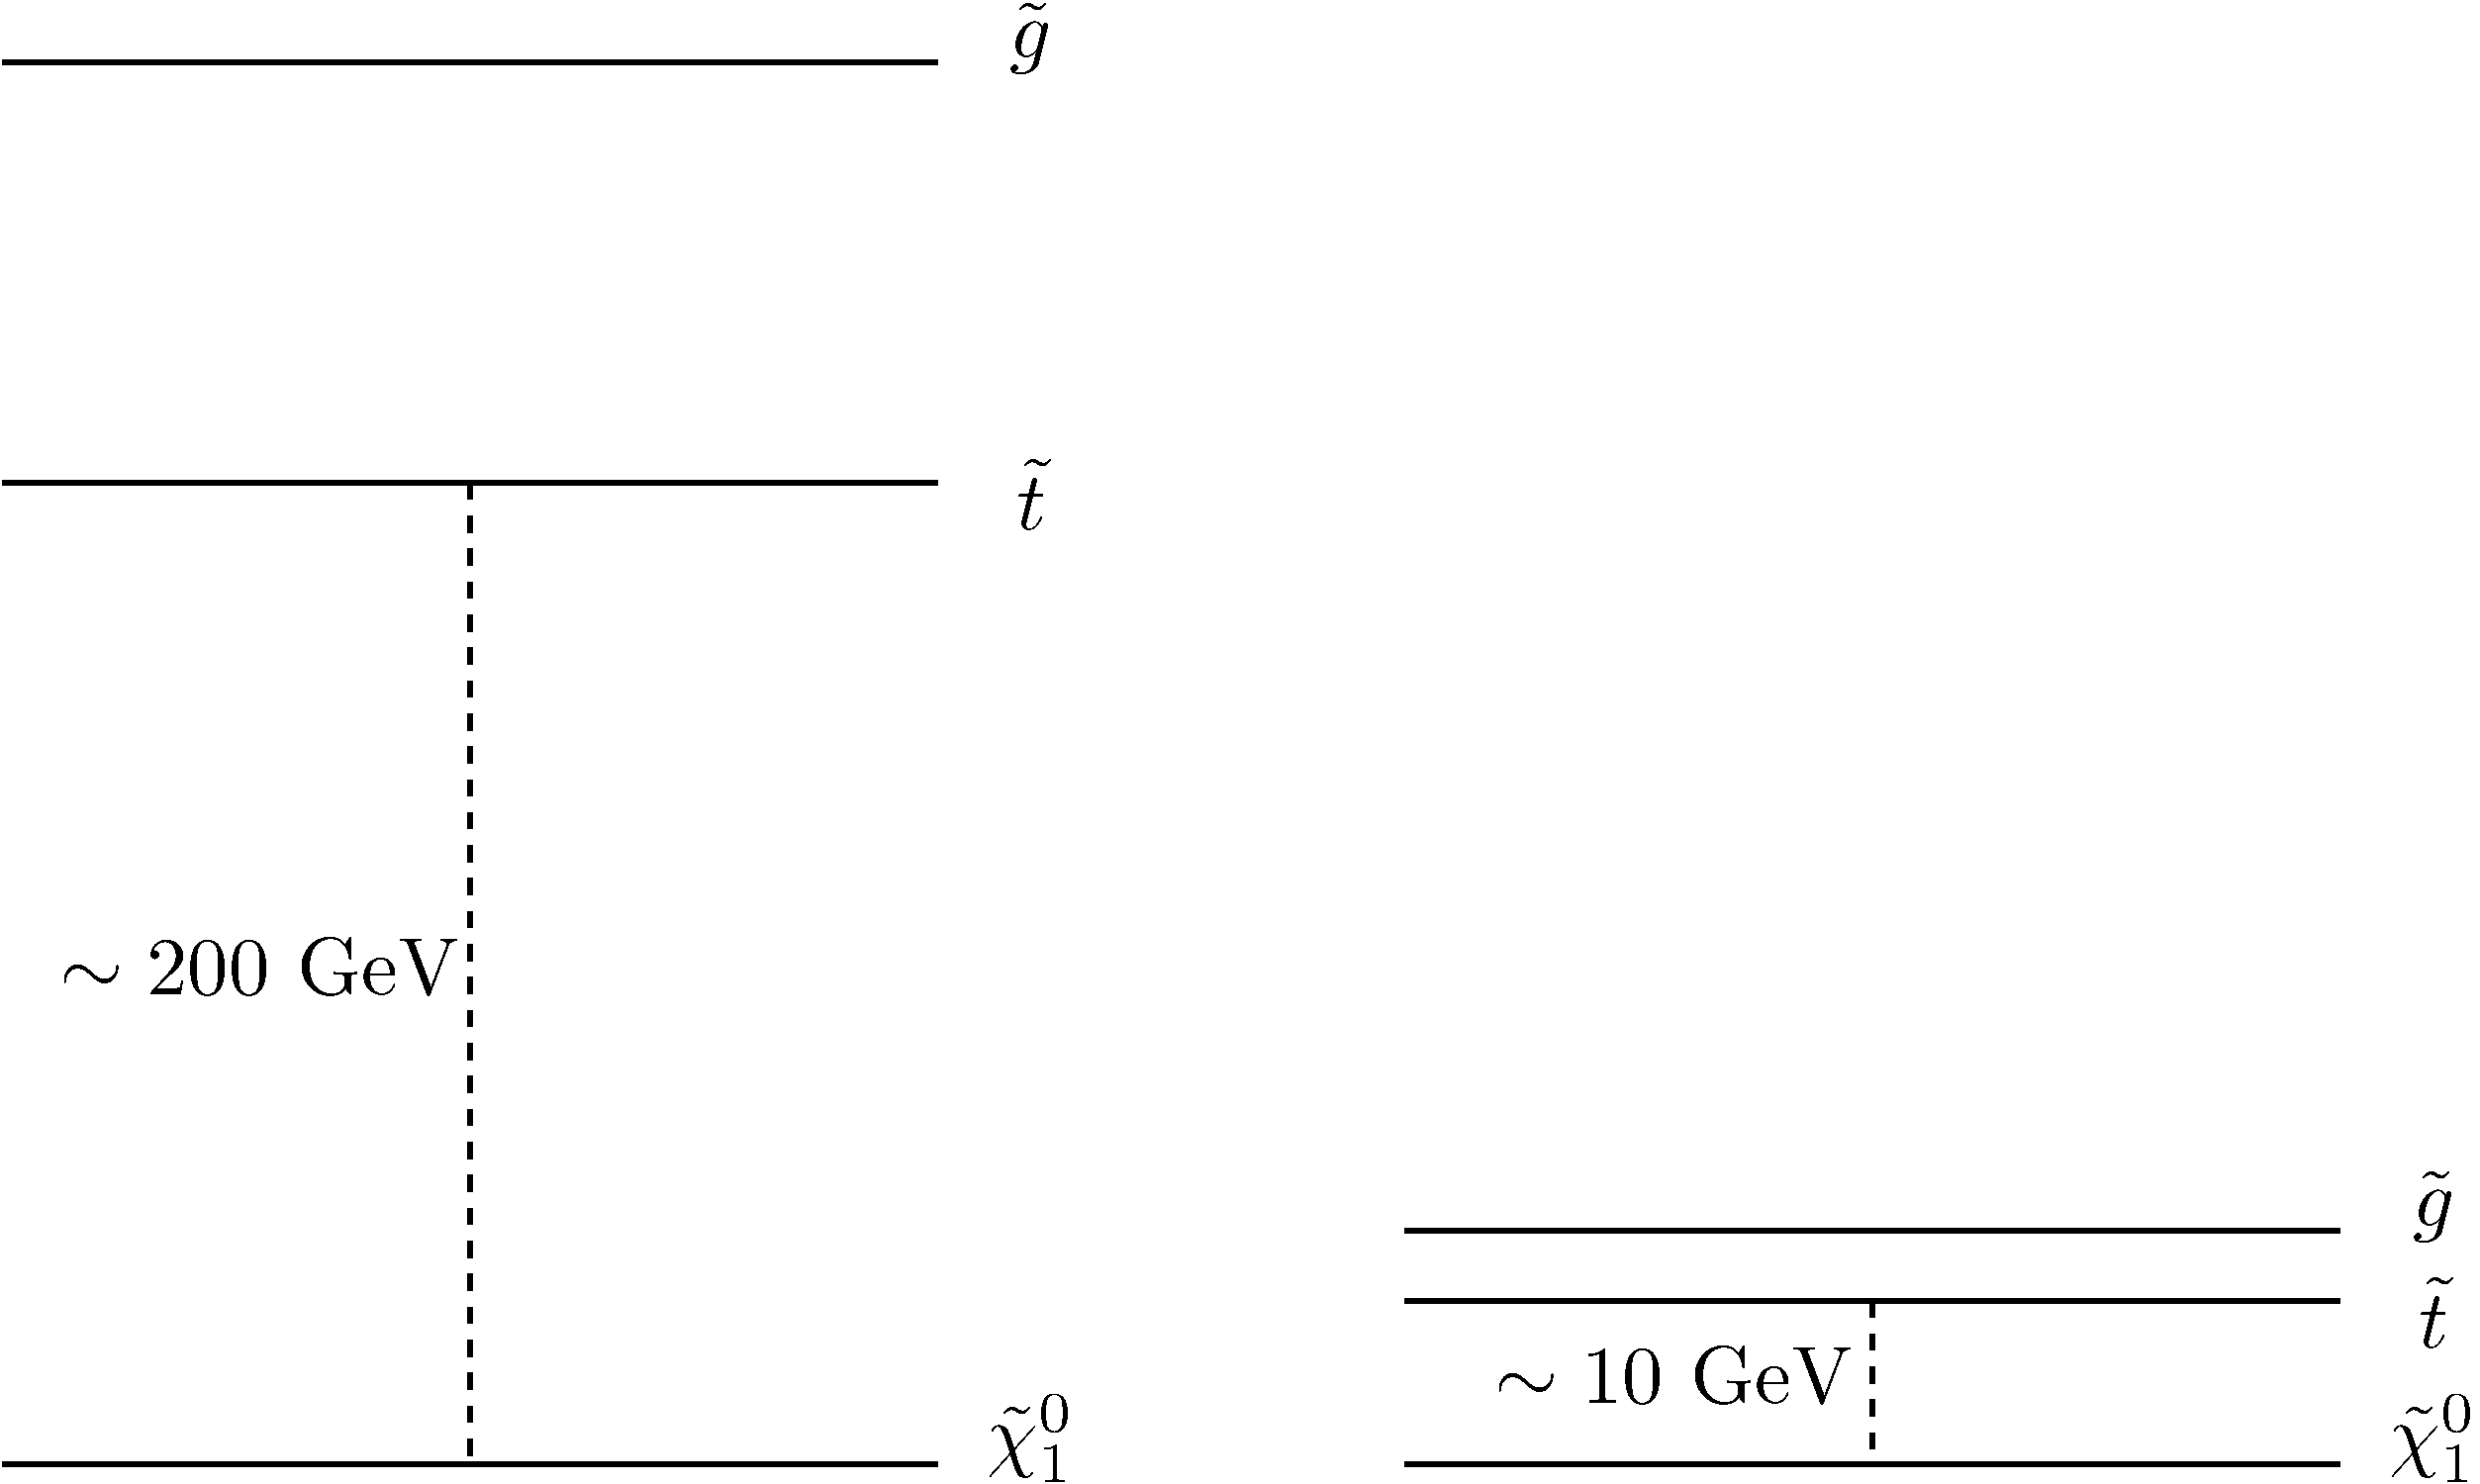
\includegraphics[width=0.7\textwidth]{Figures/theory/susyCompressedSpectra.pdf}
  \caption{An example \ac{SUSY} spectrum in the bulk region, left, and for a compressed spectrum, right. The mass difference between the \ac{NLSP} and the \ac{LSP}, here the \sTop and \chiOneZero receptively, is much reduced for the compressed scenario.}
  \label{fig:compSUSYspec}
  \end{center}
\end{figure}

% relic density
Any \ac{BSM} candidate for \ac{DM} must give the correct energy density of dark matter, which has been accurately measured by \ac{WMAP} and the Planck space telescope~\cite{WMAP2003,Planck2013}.
Any \ac{SUSY} model, if it is to explain the origin of \ac{DM} as the \ac{LSP}, must therefore give the correct \ac{DM} relic density (if nothing else is acting to increase or decrease the relic density). 
This requirement can dictate the nature of the neutralino (the \ac{DM} candidate)~\cite{CompSUSY1,CompSUSY2}.
If the neutralino is a superposition of bino states, then the relic density is too large; if it is instead a composition of higgsino or wino states, then it is too small.
However, if the neutralino is bino-like but has a few tens of~\GeV mass splitting with the lightest \sTop, the correct relic density can be achieved~\cite{CompSUSY6,CompSUSY9,CompSUSY10}.

%experimental signature
Any compressed scenario will lead to soft decay products, 
as the energy from the parent sparticle goes mostly into producing the daughter particles with little left to boost the decay products.
The question of how to efficiently select these events then presents itself -- it is very difficult to pick out events that contain only a few soft particles; 
they would be lost in the \ac{SM} electroweak, \ttbar and \ac{QCD} events.
Similarly, the \chiOneZero at the end of the decay chain will also be very soft, so \MET in each event is also small. 
Instead of looking for the decay products themselves, it is then more useful to search for 
states which are produced in association with the parent sparticles.
\ac{ISR} can lead to the emission of a high energy gluon or quark, giving a hard jet. 
It will also give a boost to the system, such that the \chiOneZero also have more momentum, and thus there will be a significant amount of \MET.
Such an event will then have a clear signature of one high momentum jet and large \MET, where the decay products are too soft to observe. 
While the production cross section of a process with an \ac{ISR} jet is of course lower than without, due to the additional factor of $\alpha_{S}$, the gain in sensitivity to the signal far outweighs the lower event yield.

%electroweak baryogenesis
% % There are also arguments for a light stop and light neutralino in the context of electroweak baryogenesis.
% Electroweak baryogenesis tries to explain the observed \ac{CP} violation in the universe, 
% by explaining the origin of the \ac{BAU}~\cite{EWKbaryogenesis}: 
% why we observe negligible antimatter in the observable universe~\cite{noAntiMatter}.
% The standard cosmological model provides accurate predictions of the abundances of light elements
% in the universe, depending on the nucleosynthesis parameter $\eta$:
% \begin{equation}
% \eta \equiv \frac{n_{b} - n_{\bar{b}}}{s},
% \end{equation} 
% where $n_{b}$ ($n_{\bar{b}}$) is the number density of baryons (antibaryons) in the universe and $s$ is the entropy density.
% The generation of $\eta$ is known as baryogenesis, and is achieved through models which have some baryon asymmetry within them. 
% If the asymmetry is generated by physics at the electroweak scale (when temperature of the universe was $\sim 10^{2}$~\GeV) it is known as electroweak baryogenesis. 
% Furthermore, as it relies upon weak scale physics, it can be tested at the~\ac{LHC}.
% For arbitrary parameters in the \ac{MSSM}, electroweak baryogenesis cannot be realized, as it cannot be in the \ac{SM}~\cite{EWKbaryogenSUSY3}. 
% Instead, the region of phase space where the top squark is light is necessary for electroweak baryogenesis~\cite{CompSUSY6,EWKbaryogenSUSY1,EWKbaryogenSUSY2}.


%The LHC limits on degenerate \gluino and \squark are strong, but when an implicit bottom-up flavour structure is considered, the \sTop and \sbottom limits significantly weaken.


\section{Decays of the top squark}

We have discussed in the previous section the importance of a light top squark for natural ~\ac{SUSY}. 
In order to optimise any search for such a light top squark, it is important to consider its decays in different regions of parameter space~\cite{CompSUSY7,CompSUSY8}.

For the case when the mass difference between the top squark and the \ac{LSP} is greater than the mass of the top quark, 
$m_{\sTop} - m_{\chiOneZero} > m_{t}$, 
the dominant decay mode is simply 
$\sTop \rightarrow t \chiOneZero$.
The Feynman diagram for \sTop pair production followed by this decay is shown in Fig.~\ref{fig:t2tt}.

However, when the mass difference is less than the top quark, 
$m_{\sTop} - m_{\chiOneZero} < m_{t}$, 
things become more complicated. 
While the mass difference is above the mass of the W, 
$m_{\sTop} - m_{\chiOneZero} > m_{W}$, 
the three body decay mode $\sTop \rightarrow W b \chiOneZero$ dominates, as the W can be produced on-shell.
As the mass difference becomes smaller still, 
$m_{\sTop} - m_{\chiOneZero} < m_{W}$,
both the flavour changing neutral current decay 
$\sTop \rightarrow c \chiOneZero$ 
and the four body decay 
$\sTop \rightarrow b \chiOneZero f \bar{f}'$ can occur, where $f$ is any fermion.
Examples of Feynman diagrams that contribute to these are shown in Fig.~\ref{fig:stopDecays}.
While the precise branching fraction of these decay modes is rather model dependent, it is usually assumed that due to phase space arguments, the four body decay is suppressed and $\sTop \rightarrow c \chiOneZero$ dominates~\cite{CompSUSY7}.
Figure~\ref{fig:stopDecayMassPlane} summarizes the decays of the top squark, showing the relevant decay for the different kinematic regimes of \sTop and \chiOneZero mass.

\begin{figure}[t!]
  \begin{center}
  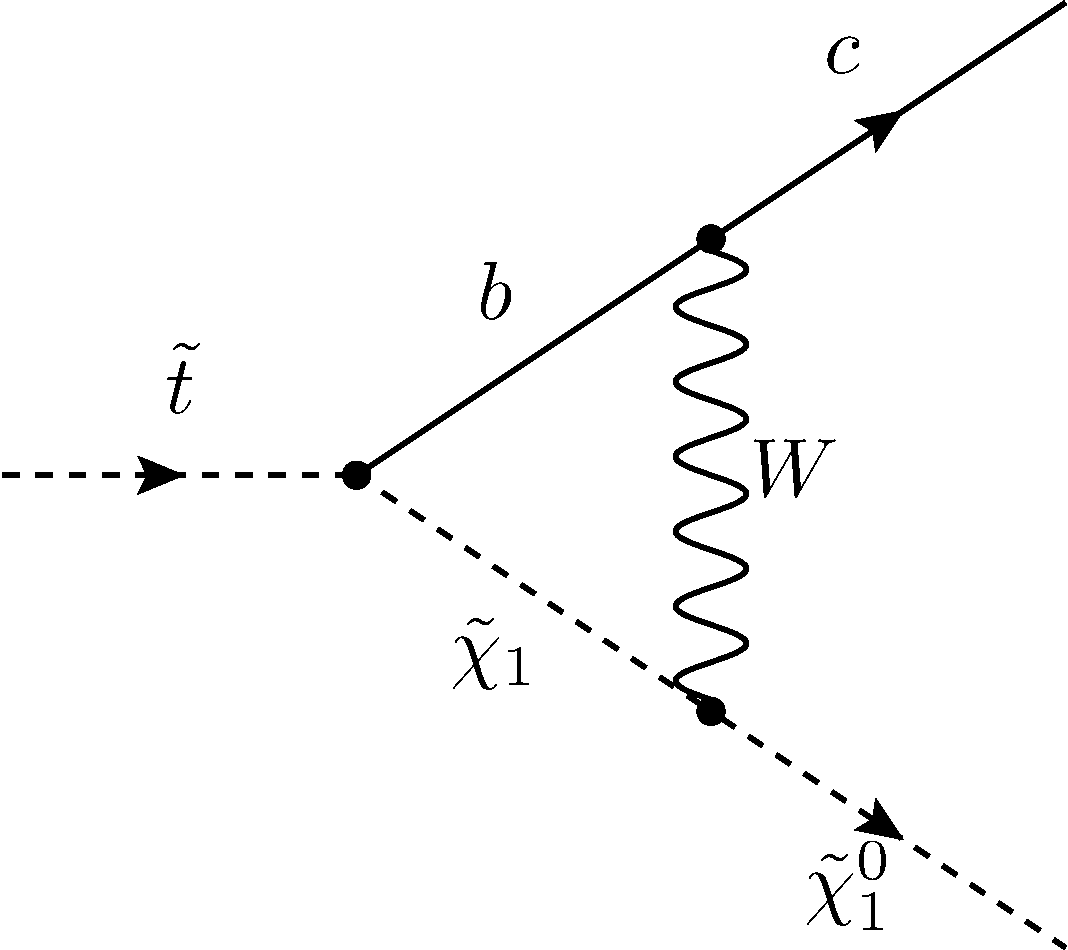
\includegraphics[width=0.3\textwidth]{Figures/theory/stop2bodydecay.pdf}
  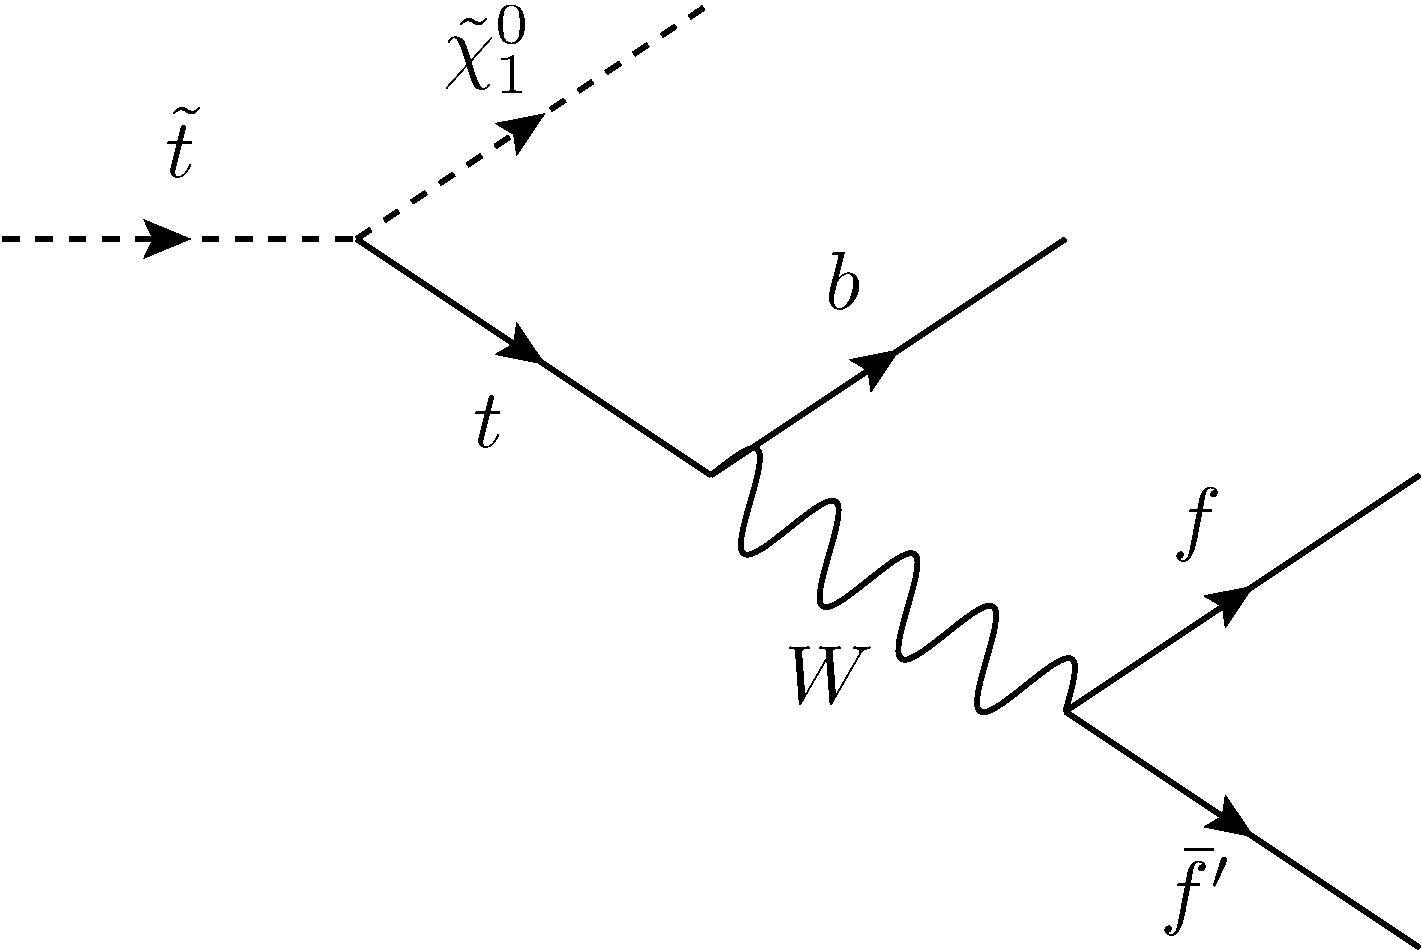
\includegraphics[width=0.4\textwidth]{Figures/theory/stop4bodydecay.pdf}
  \caption{Feynman diagrams to show two contributing processes to the decays of the top squark: $\sTop \rightarrow c \chiOneZero$ (left) and $\sTop \rightarrow b \chiOneZero f \bar{f}'$ (right).}
  \label{fig:stopDecays}
  \end{center}
\end{figure}
 

\begin{figure}[t!]
  \begin{center}
  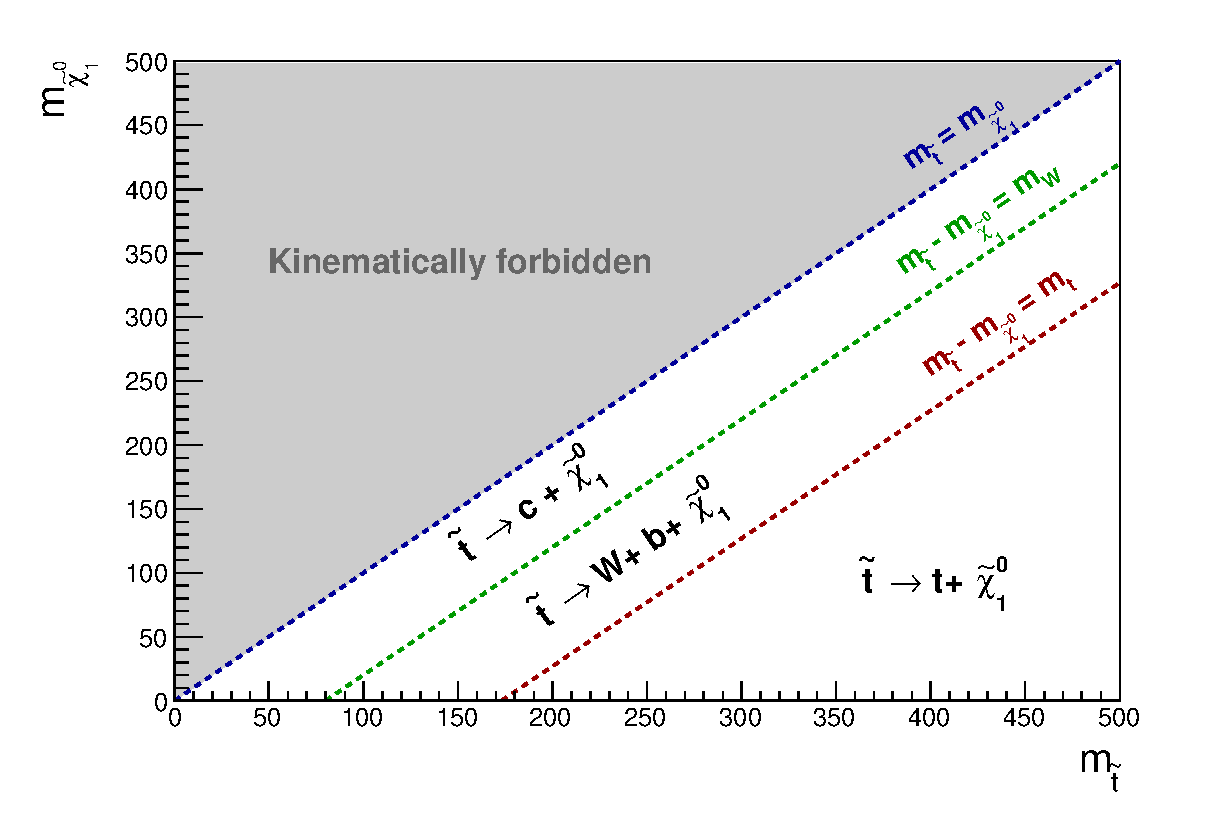
\includegraphics[width=0.7\textwidth]{Figures/theory/stopMassPlane}
  \caption{Phase space of the top squark and LSP. The grey region is kinematically forbidden: 
  $m_{\chiOneZero} > m_{\sTop}$ is at odds with the \ac{LSP} definition. 
  The coloured dotted lines and labels define each kinematic region, and the dominant \sTop decays are shown, where we have neglected the four body decay in the region where $m_{\sTop} - m_{\chiOneZero} < m_{W}$.}
  \label{fig:stopDecayMassPlane}
  \end{center}
\end{figure}

In light of the arguments for searching for compressed \ac{SUSY}, particularly in the third generation, 
Chapters~\ref{chap:sus13009} and~\ref{chap:parkeddata} will describe searches for light stops decaying to a charm quark and a neutralino, using events with a monojet topology.
